When studying temporal structures in neural dynamics, the definition of the time references is a key first point. In the computational analysis in the previous section, the time reference to define the intervals were first and last spike of each burst. In that case, as in the case of interneurons in \textit{C. maenas} the CPG phases are directly related with the bursting activity of these neurons and the burst can be consistently defined by the first and last spike. However, in the case of \textit{Lymnaea stagnalis}, activity is usually characterized using recordings from both interneurons and motoneurons \parencite{elliott_interactions_1985, staras_pattern-generating_1998, benjamin_distributed_2012}. This leads to the need of a combination of burst references to characterize the phases of the CPG based on the time intervals cycle by cycle. Thus, for this analysis, we will consider the three phases in the CPG, protraction, rasp and swallow, that are associated mainly to N1M, N2v and N3t neurons. Since it is not always possible to record those neurons at the same time (specially N2v that is in the ventral side), we will define them by a combination of interneurons and motoneurons following their activity at each phase. For example, in Figure \ref{fig:example lymnaea phases recording} the three phases in the  CPG are marked by a colored background over the recording, note how it can be delimited by the neurons in the circuit but some of the motoneurons cover several phases, as it is the case of B4 in panel a) or B3 in panel b). Also phases can be defined by the first and last spike, as it is the case for phase N3 and neuron B8, but in other cases as the phase N2, the reference is the hyperpolarization of some neurons, such as the strong inhibition visible in neuron B5 in panel b). Also, depolarization of some neurons carry relevant information, since for example in the case of B1 the "bumps" visible represent the N1 phase, by the connection between N1M and B1. Therefore, to characterize the time sequences in the feeding CPG, we need compound references from several neural recordings that can be summarized as in Table \ref{table:cpg ref intervals}. Note that, although different time references must be taken into account when reaching conclusions about the time-interval restrictions and analysis, all possible intervals conforming each cycle between the neurons are taking into account in this analysis (see \ref{subsec:intervals}), so the restrictions and analysis are still relevant. The reference to define each time-interval for each recording are described in section \ref{subsec:methods experimental intervals}.


\begin{figure}[bth!]
	\centering
	\begin{minipage}[b]{\textwidth}
		\makebox[0pt][l]{\hspace*{-130pt}\text{a)}}\\
		\centering
		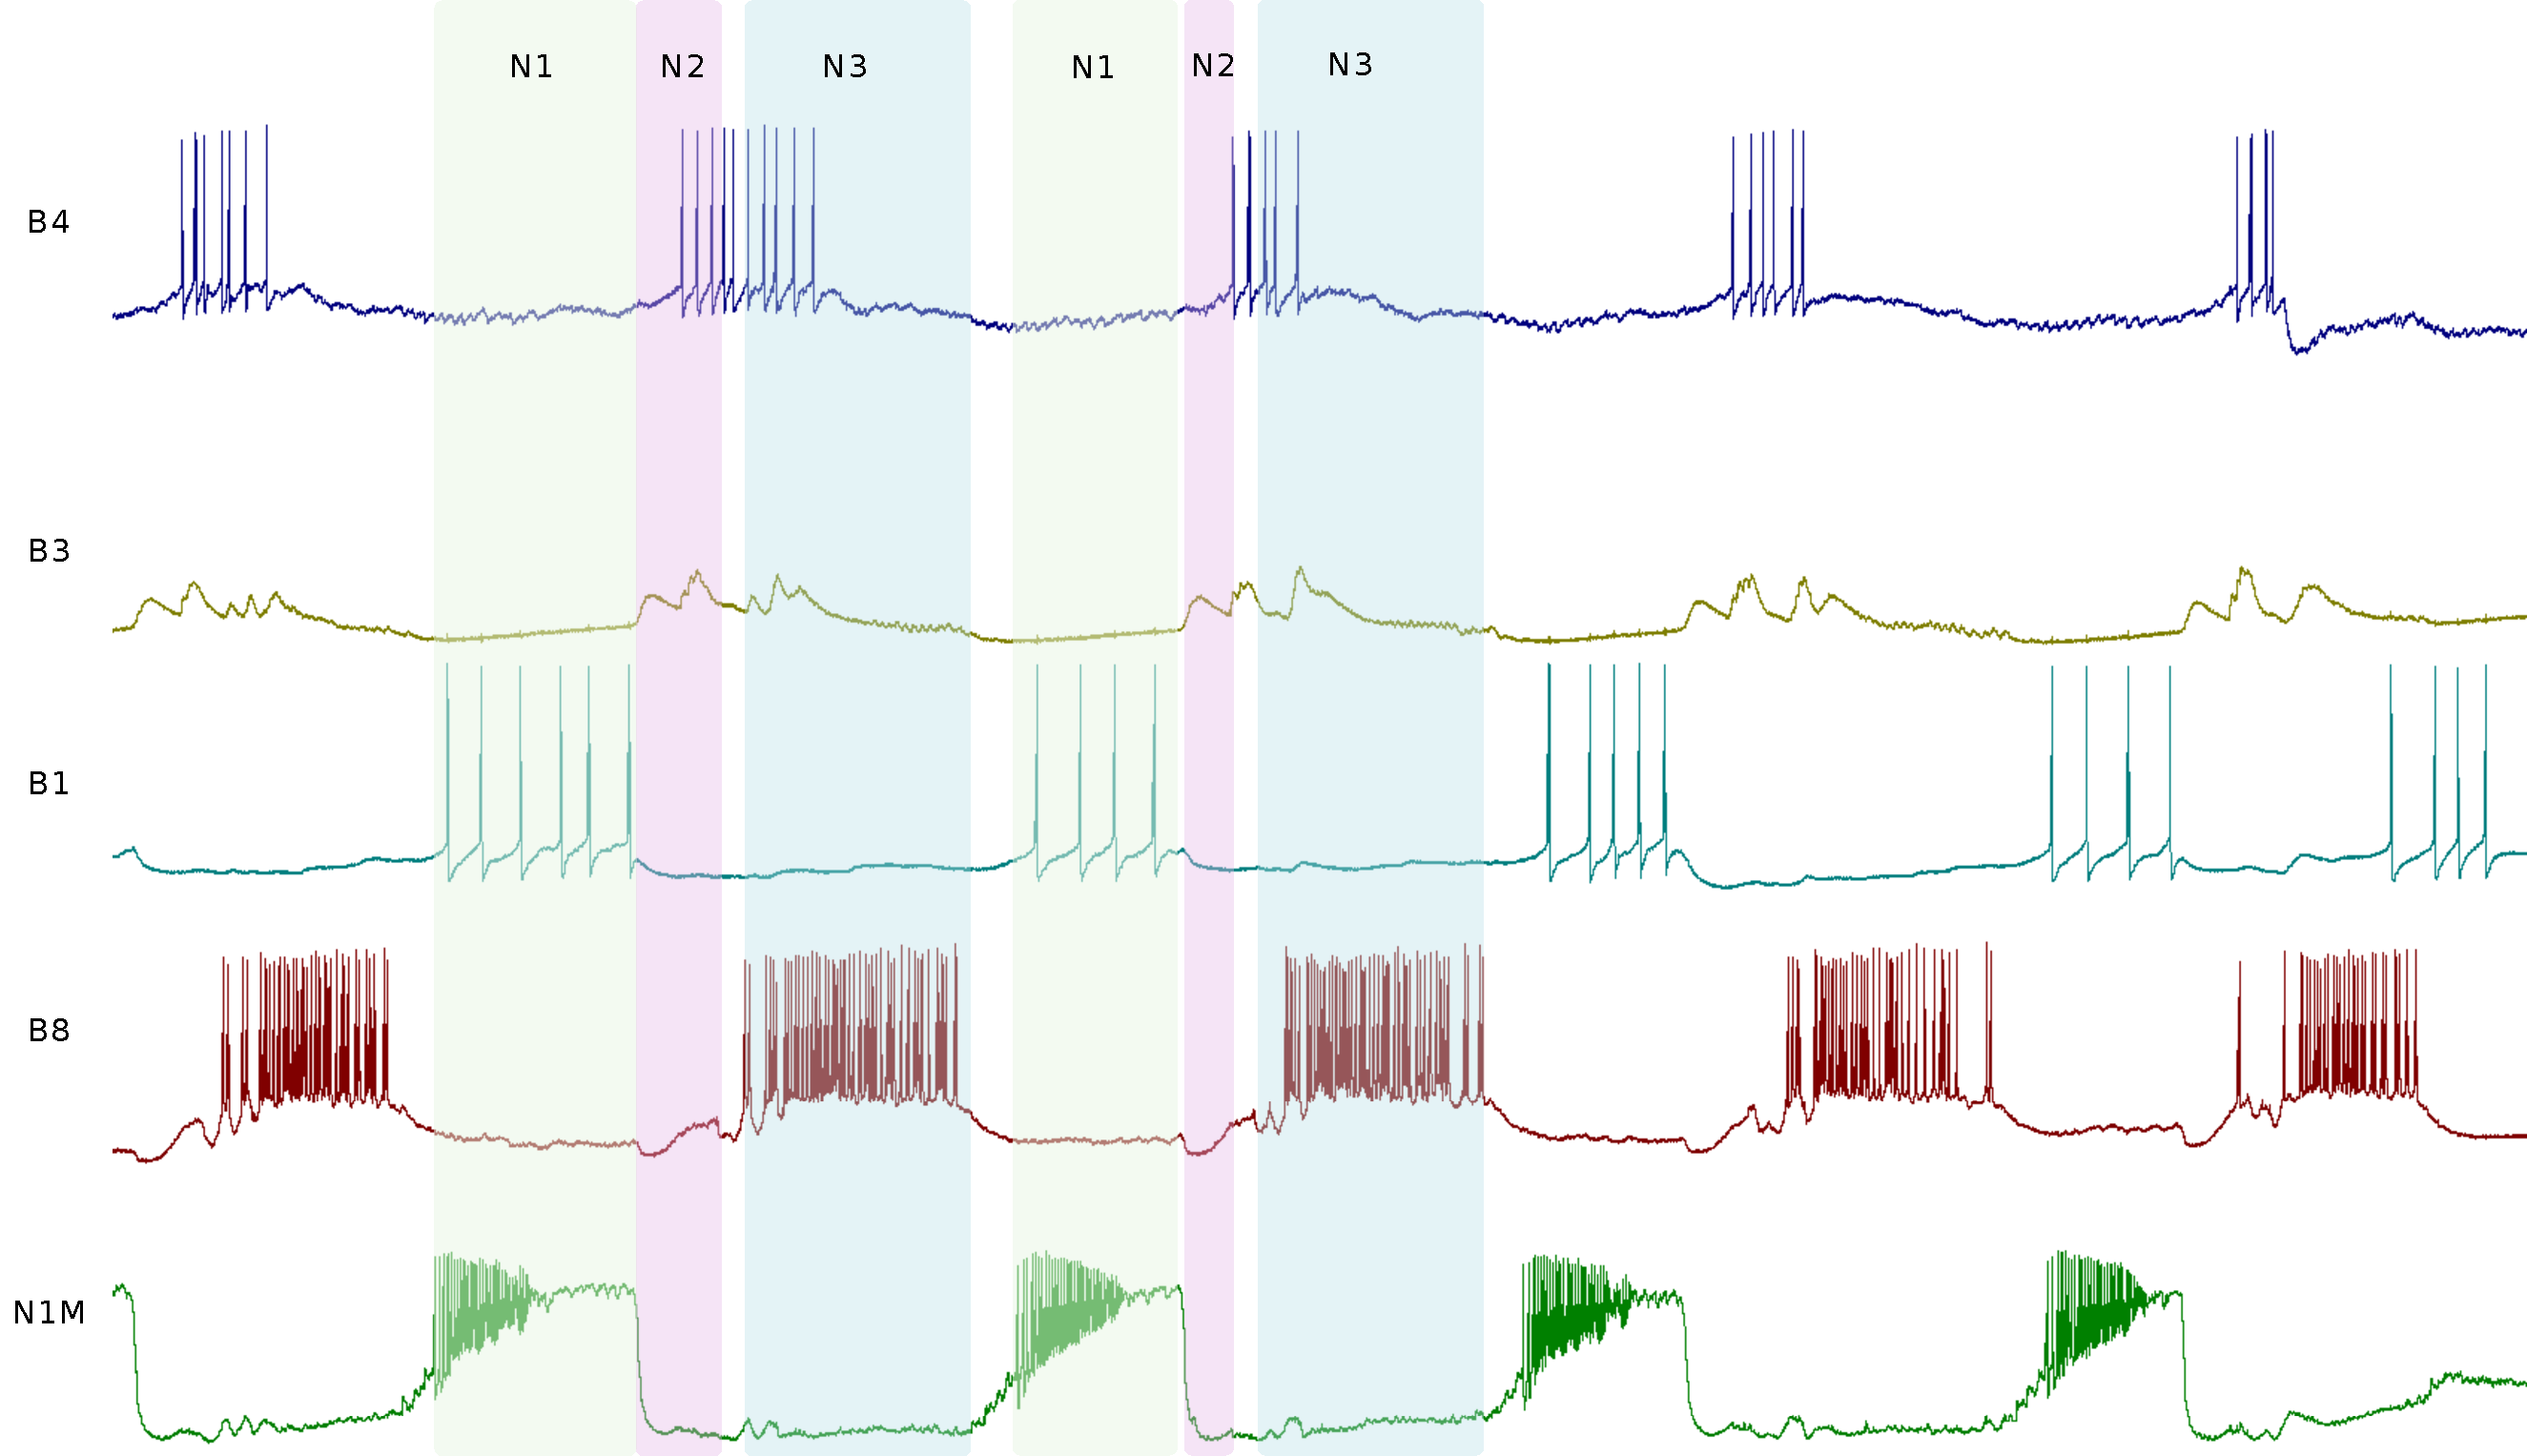
\includegraphics[width=0.9\textwidth]{img/invariants/example_phases_1.pdf}
	\end{minipage}
	\vspace{20pt}
	\begin{minipage}[b]{\textwidth}
		\makebox[0pt][l]{\hspace*{-130pt}\text{b)}}\\
		\centering
		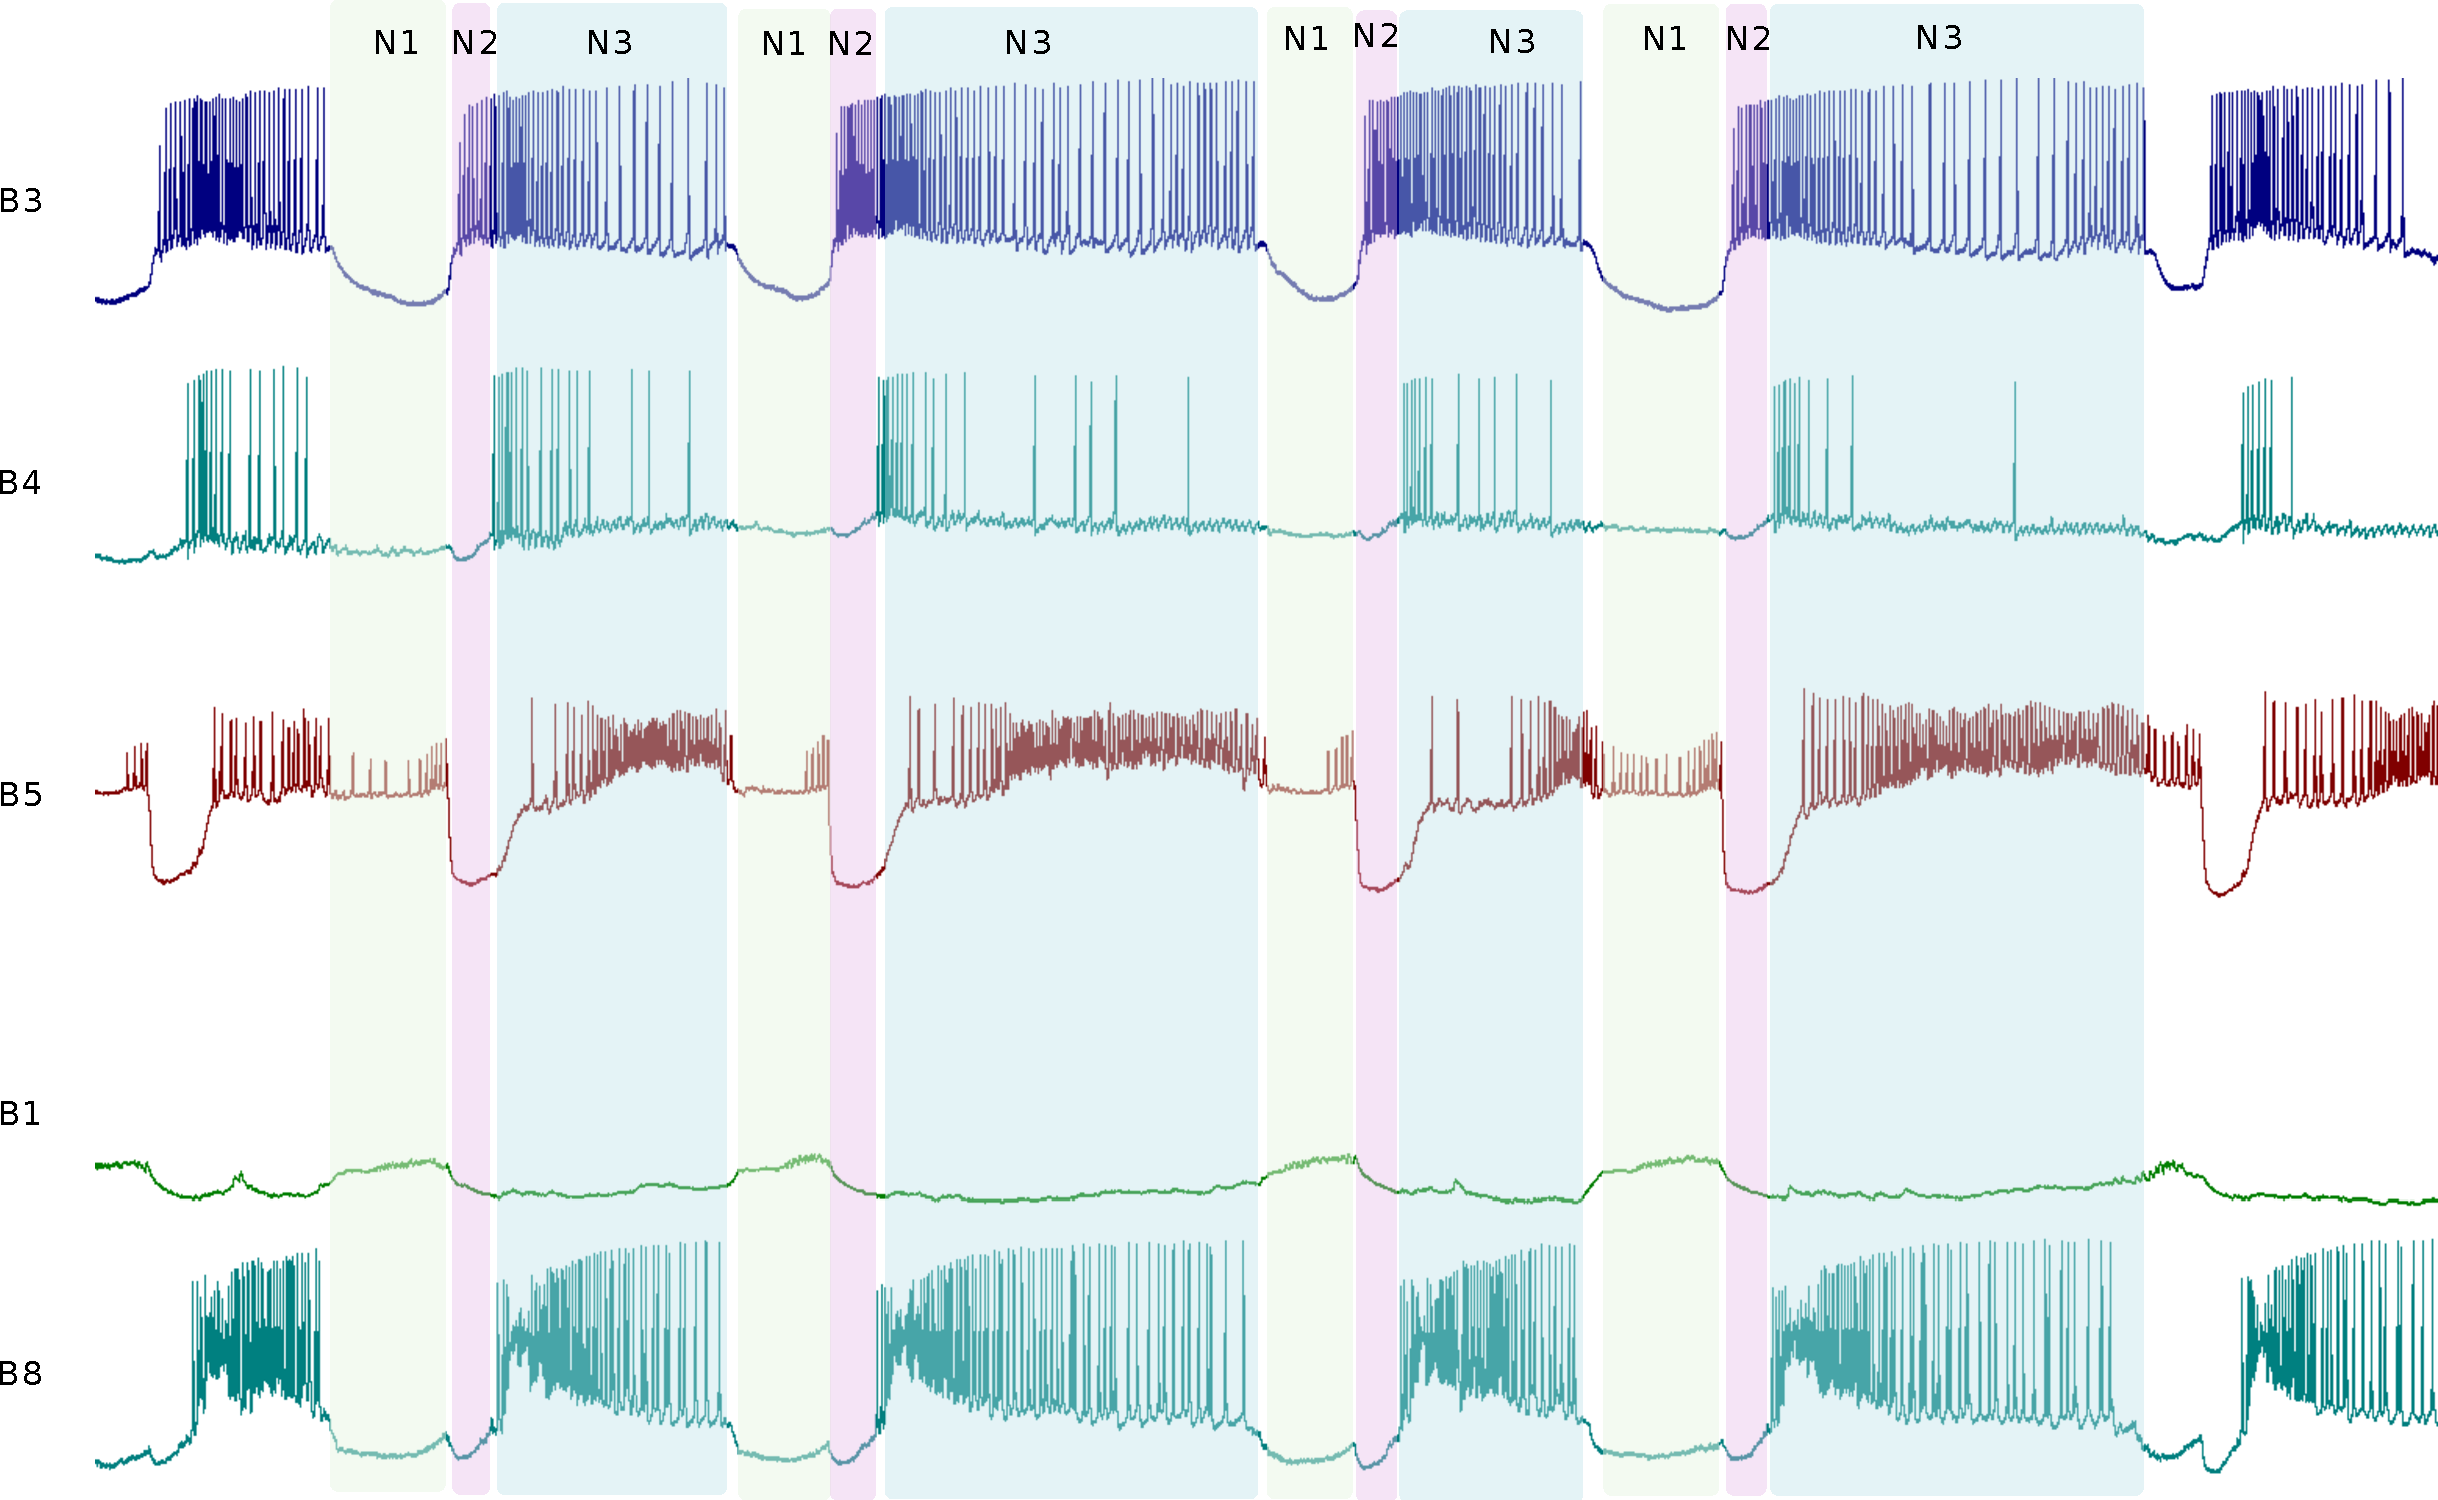
\includegraphics[width=0.9\textwidth]{img/invariants/example_phases_2.pdf}
	\end{minipage}
	\caption{Delimitation of phases in the feeding CPG of \textit{Lymnaea stagnalis} based on different recordings. Panel a) intracellular recordings for motoneurons B4,B3,B1 and B8 and the interneuron N1M. Phases are delimited by N1M and B1, that have the same activation time for phase N1, the inhibition of N1M and the start of the depolarization in B8 for phase N2 and the first and last spike of burst B8 for phase N3. Panel b) intracellular recordings for motoneurons B3,B4,B5, B1 and B8. Phases are delimited by B1 depolarization for phase N1, the strong inhibition of B5 for phase N2 and the fisrt and last spike of burst B8 for phase N3.}
	\label{fig:example lymnaea phases recording}
\end{figure}

Another key point in the study of the feeding CPG of \textit{L. stagnalis} is that the generation of the rhythm is a combined action of different cells \cite{benjamin_distributed_2012}, not only interneurons but also motoneurons have a role in the activation \parencite{staras_pattern-generating_1998} and modulatory neurons in the buccal and cerebral ganglia are involved in the rhythm. All these factors affect the rhythm and thus the neuronal sequential activation and how variability is distributed among the different intervals cycle by cycle. Also, not all the neurons are involved every time the rhythm is active, and that gives also information about the different contexts in which the rhythm is taking part. For example, the rhythm can be activated by the presence of food or sucrose stimulation, in which case the animal needs to initiate the activity and ingest food, the rhythm is started by the stimulation of the lip nerve that also stimulates N1M. Also, even at the absence of food but when the animal is hungry, the CPG can be activated, in this case with a strong role of N3t as modulator. The modulation of the rhythm is also a key aspect and modulatory neurons as SO or CV1a control the rhythm after its initiation, showed to have distinct alternative roles in the activity \parencite{kemenes_multiple_2001}. 

\begin{figure}[bth!]
	\centering
	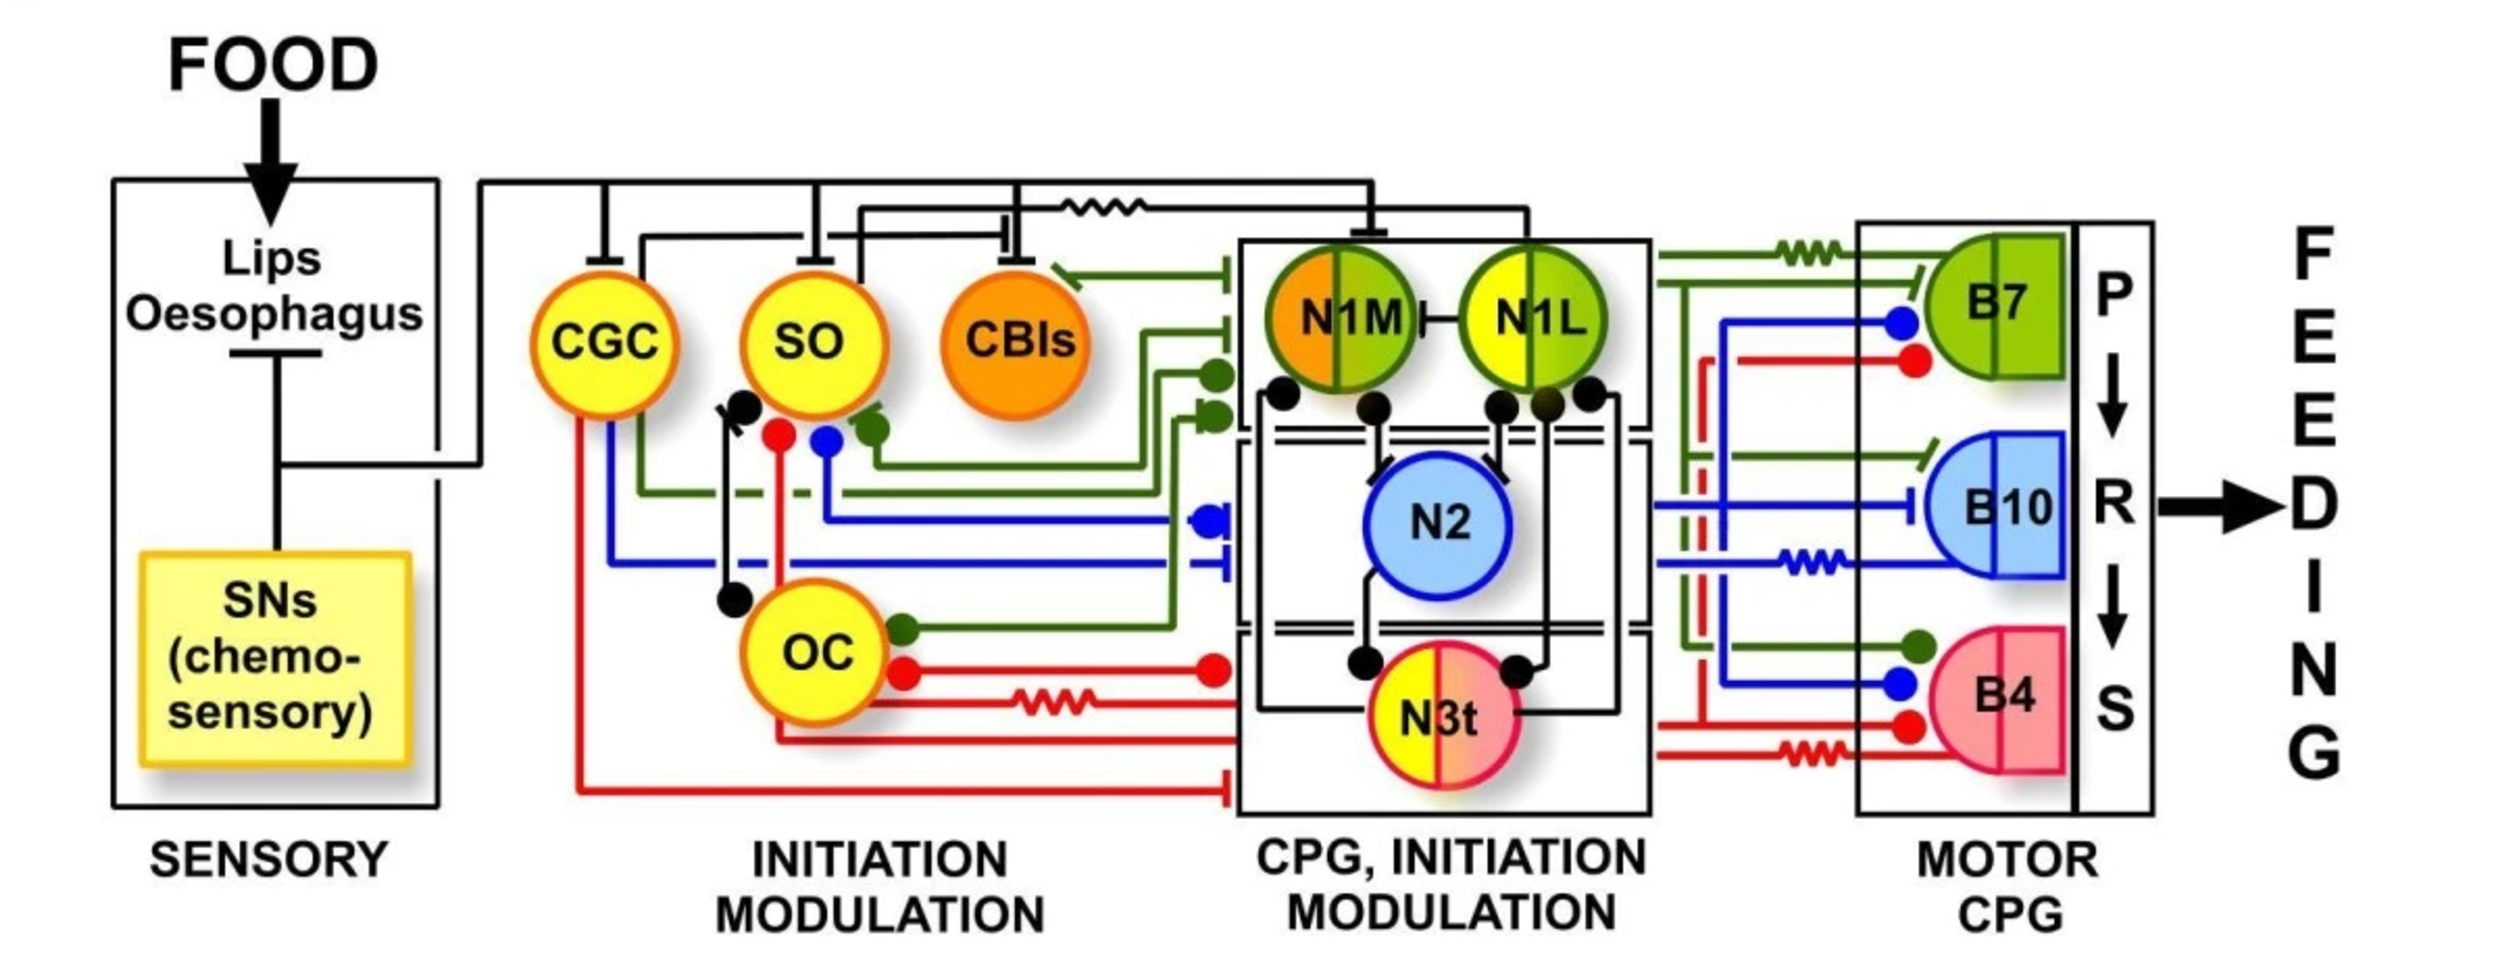
\includegraphics[width=\textwidth]{img/invariants/distributed_benjamin_2012.pdf}
	\caption{Representation of the distributed system of the feeding CPG. Dots indicate inhibitory chemical synapses, bars excitatory chemical synapses and resistor symbols electrotonic (electrical) synapses. Colors indicate the function of the neuron classified in modulatory or initiator (yellow and orange, respectively) and the three phases protraction, rasp and swallow (green, blue and red, respectively). From left to right food detection represented by Lips that stimulate CGC, SO CBIs and N1M neurons and initiate the rhythm. The ongoing activity is then modulated by those neurons but also by OC neurons and N1 and N3t neuron. Some examples of motor neurons are represented on the right side of the panel, associated to each feeding phase. This figure was adapted from Panel C from Figure 1 in \cite{benjamin_distributed_2012} (work under license \href{http://creativecommons.org/licenses/by/2.0}{Creative Commons Attribution})}
	%	Synaptic connectivity and functions of neurons in the feeding circuit. Modulatory function is indicated by yellow and initiating function by orange. CPG interneurons and motoneurons active during the three phases of the feeding rhythm are indicated by green (P = protraction), blue (R = rasp) and red (S = swallow). Neurons labeled with two colors have two functions. Dots indicate inhibitory chemical synapses, bars excitatory chemical synapses and resistor symbols electrotonic (electrical) synapses. This figure emphasizes the point that many of the neurons have more than function in the feeding network. See Abbreviations for all definitions of neuron types.
	\label{fig:feeding distribution}%
\end{figure}

%Benjamin2012    One of the central controllers of
%spontaneous feeding is the N3t CPG interneuron and
%this cell is involved in mediating the effects of hunger
%and satiety. As was described earlier, the N3ts fire toni-
%cally to inhibit the N1M cells and the rate of this tonic
%activity determines the level of activity in the whole feed-
%ing CPG. By comparing the rates of firing in isolated
%ganglia it was found that the N3t firing frequency was
%higher in satiated compared with starved snails and that
%this was inversely correlated to the frequency of sponta-
%neously fictive feeding cycles [4]. 

%kemenes 2001
%CV1a by modulating motoneuron burst duration and SO by setting the frequency of the ongoing rhythm

In this section we will analyze and describe different examples of experiments for the isolated ganglia with intracellular recordings under: spontaneous activity, SO-driven activity spontaneous and induced, medium lip nerve stimulation induced activity and CV1a-driven induced activity.



\subsection{Invariants in spontaneous activity}
The spontaneous activity here refers to intracellular recordings of the buccal ganglia after the isolation of the CNS with no chemical or electrical induced stimulation. In that case, since the CPG is able to maintain the activity in an autonomous manner, it keeps the motor activity as if the CNS was not isolated. In this case, although the characterization of the sequential dynamical invariants can be done, their possible functionality association is more complicated, since the context of the movement origin is lost. The study of these sequential restriction in artificial stimulation context can help classify this spontaneous activity, even when the rest of the system is not available. 

Here we analyze three examples of the spontaneous activity, in these cases we do not know what was the source or context for the feeding activation, but there are differences between the three experiments in their dynamical invariants. The case with the strongest linear correlation is the first example showed in Fig. \ref{fig:prep2 invariants}, where the N3 burst duration and the associated intervals covering N3 phase (N2N1 interval, N3N1 interval, N2N1 delay) hae a strong linear correlation with the period ($R^2 > 0.9$). This is also clear in the variability boxplot, where the variability distribution of the period is really similar to N3 burst duration, N2N1 interval, N3N1 interval, N3N2 interval and N2N1 delay, and the rest of the intervals are not similar to the period's. This unsimilarity in variability is also important, since while those intervals have a strong linear correlations, some other intervals have no relation, all have $R^2 < 0.1$. Seeing the recording of this example (first row in Fig. \ref{fig:prep2 invariants}) the N3 neuron has long periods of tonic firing (that were excluded from the time-interval relations), and indicate that the spontaneous activity, was lead by N3 neuron, associated in the literature with spontaneous activity in satiated animals, where the N3t is tonically firing producing long periods of silence interrupted by short rasps \parencite{staras_loss_2003,benjamin_distributed_2012}.

However, in the following examples the variability distribution is different, in the example in Fig. \ref{fig:prep3 invariants} we can appreciate a distribution of the variability between N1 and N3 phases, observed in the boxplot, specially in the burst durations, but also in the linear regressions, that, although they have low values, we can observe linear tendencies, specially in combined intervals such as N3-N2 interval. What is a common characteristic with the previous example is the unrelated intervals to the period, since N2 burst durations and other time-intervals associated to N2 phase (N2N3 delay, N1N2 delay) have a $R^2 < 0.1$. These intervals also remain unrelated to the period in the third example, showed in \ref{fig:prep1 invariants}, where N2 and N2N3 delay have similar $R^2$ values. In that last case, however, the variability is mostly in N1 phase. Again, the linear correlations with the period are in combined periods, usually the ones involving N1 and N3 phases: N31N1 interval, N2N1 delay, N3N1 delay; this points to the distribution of variability between those two phases. Also, the fact that the combined intervals have much stronger linear correlations, is affected by the time references in these intervals, that since the first and last spike of the burst are not always well-defined, intervals as the delay give us more information than in other cases such as the model study in the previous section \ref{sec:CPG model}.

%In the absence of food, particularly in satiated animals (see the Hunger and satiety section, below), snails show long periods of quiescence with only occasional spontaneous rasps. It has been shown that the quiescence is due to tonic inhibition of the N1Ms by the N3ts [4]. During quiescence the N3ts fire continuously and via the strong inhibitory connection prevent N1M plateauing (Figure 4B, left). When sucrose is applied to the lips (Figure 4A), the N3ts are hyperpolarized (Figure 4C) reducing the level of tonic inhibition to the N1M and this has a permissive effect in allowing the N1M to plateau (Figure 4C). Thus during the sucrose-driven feeding pattern, the N3ts fire rhythmically as part of the feeding CPG (Figure 4B, right) due to the reciprocal inhibitory synaptic connections with the N1Ms. Thus N3ts have a role in modulating the feeding network as well as being part of the CPG (Figure 1C).


\begin{figure}[htbp]
	\centering
	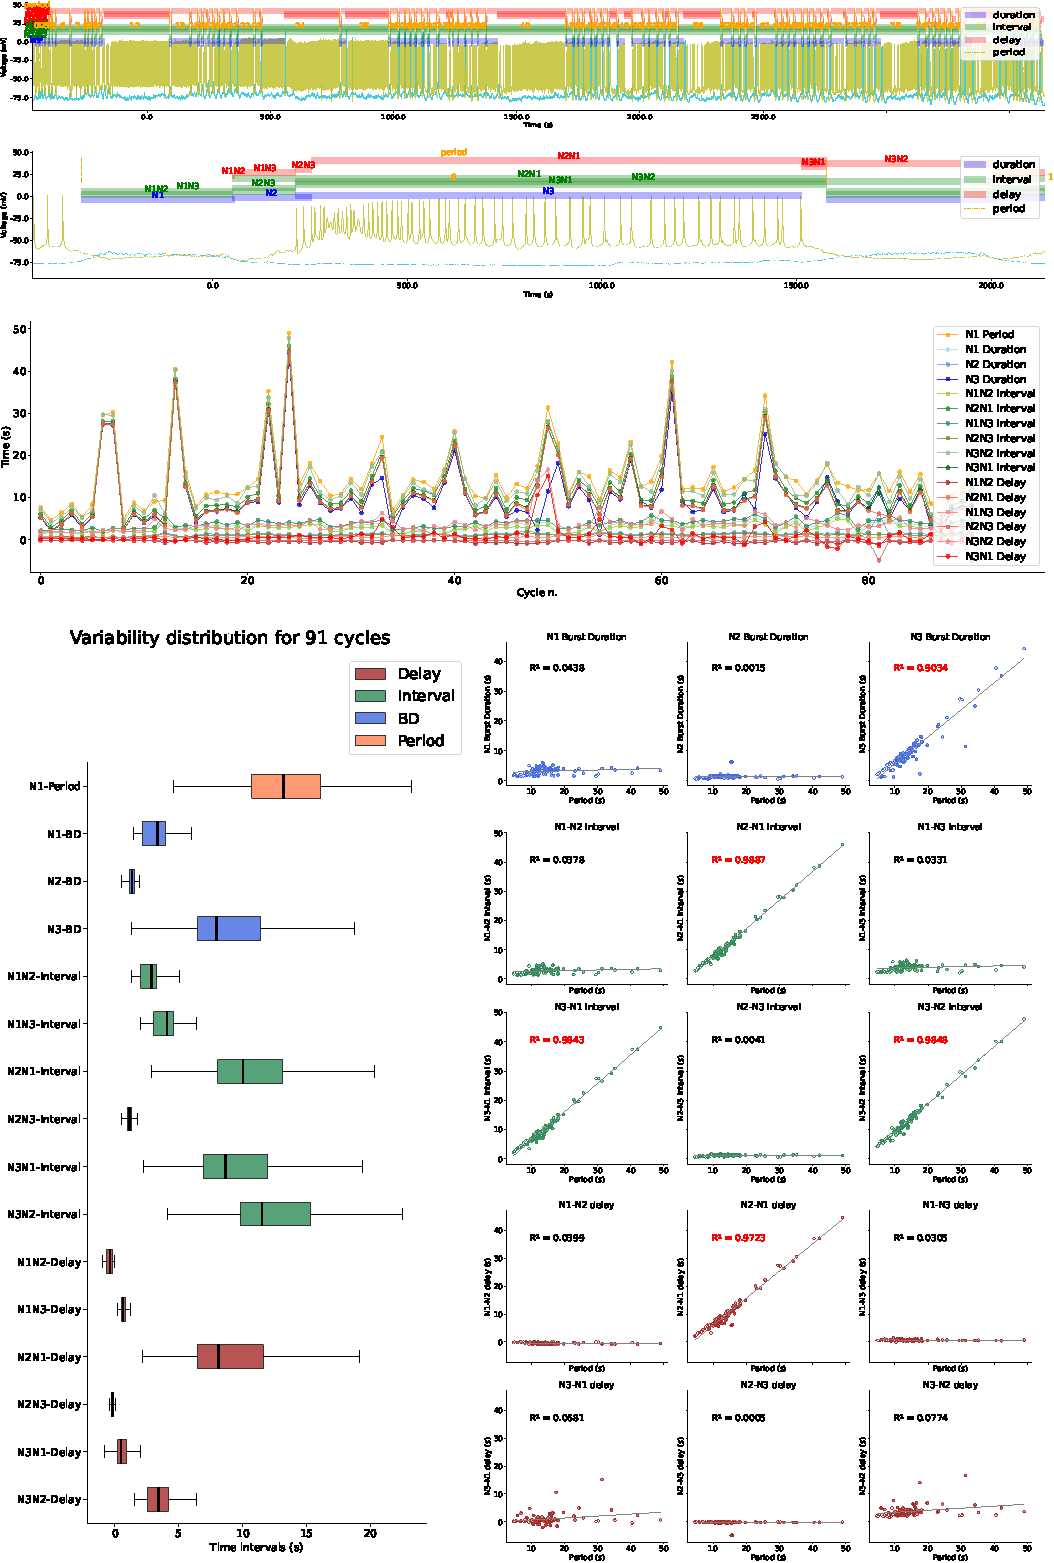
\includegraphics[width=0.9\textwidth]{./img/invariants/data/SUSSEX/prep2/images/3phases/panel_with_intervals.pdf}
	\caption{\textbf{Spontaneous case 1}: Panel of intervals distribution and dynamical invariants for the three phases in the CPG for spontaneous activity.}
	\label{fig:prep2 invariants}
\end{figure}

\begin{figure}[htbp]
	\centering
	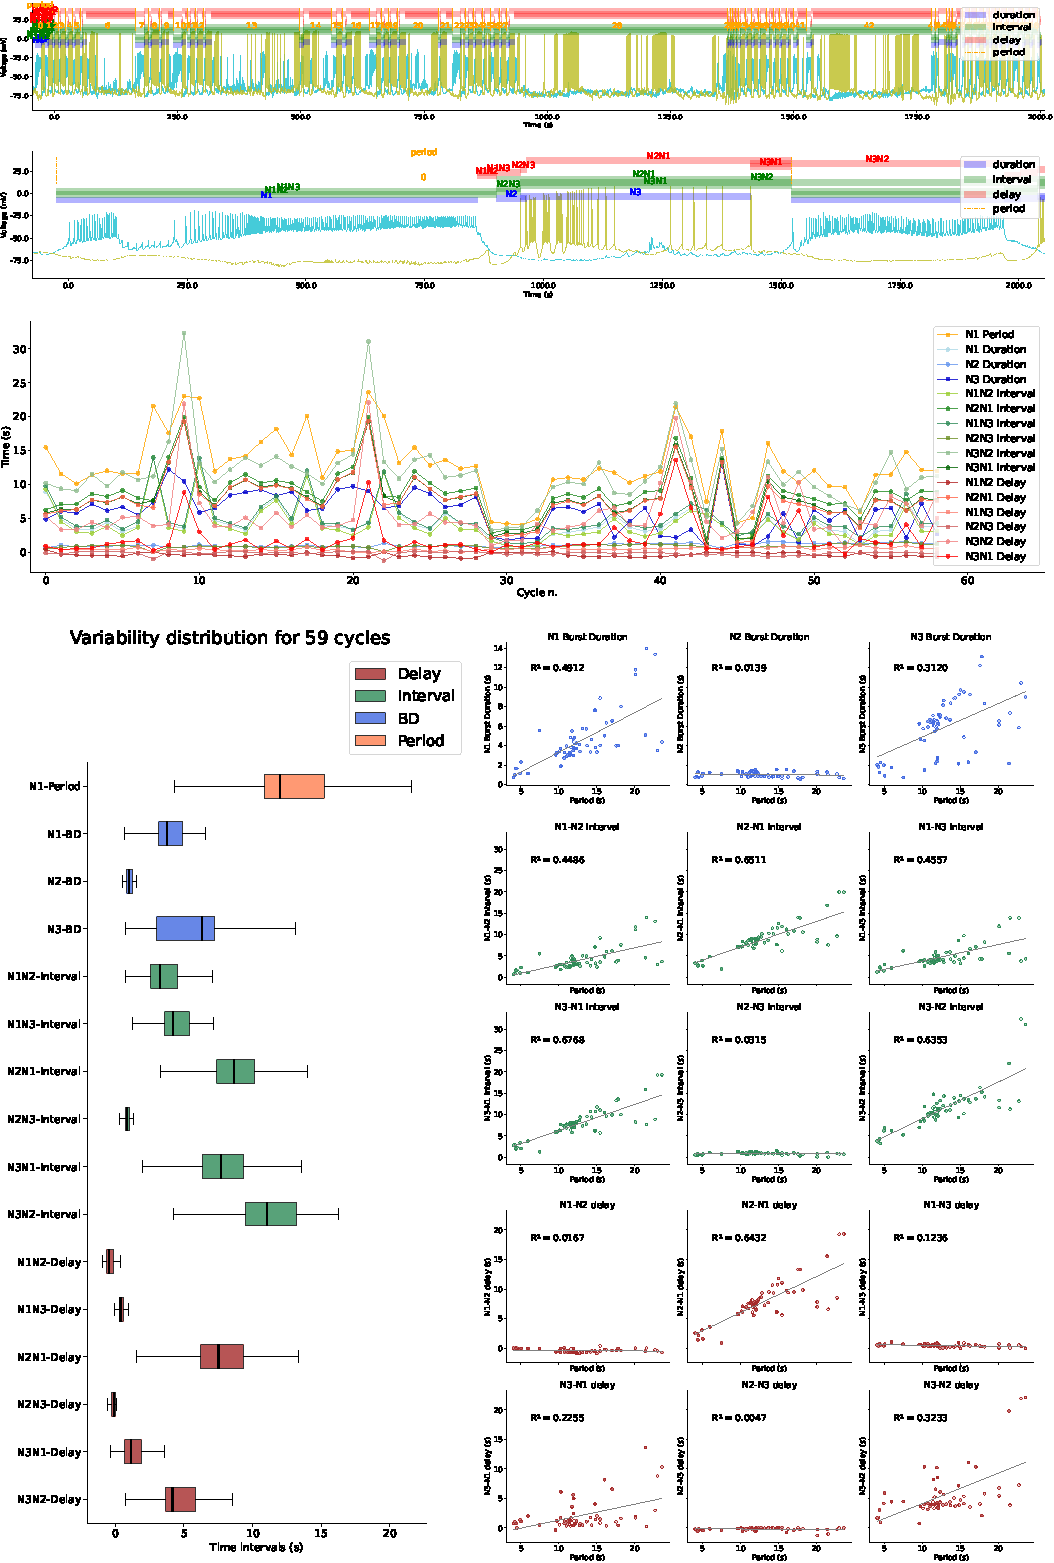
\includegraphics[width=0.9\textwidth]{./img/invariants/data/SUSSEX/prep3/images/3phases/panel_with_intervals.pdf}
	\caption{\textbf{Spontaneous case 2}: Panel of intervals distribution and dynamical invariants for the three phases in the CPG for spontaneous activity.}
	\label{fig:prep3 invariants}
\end{figure}

\begin{figure}[htbp]
	\centering
	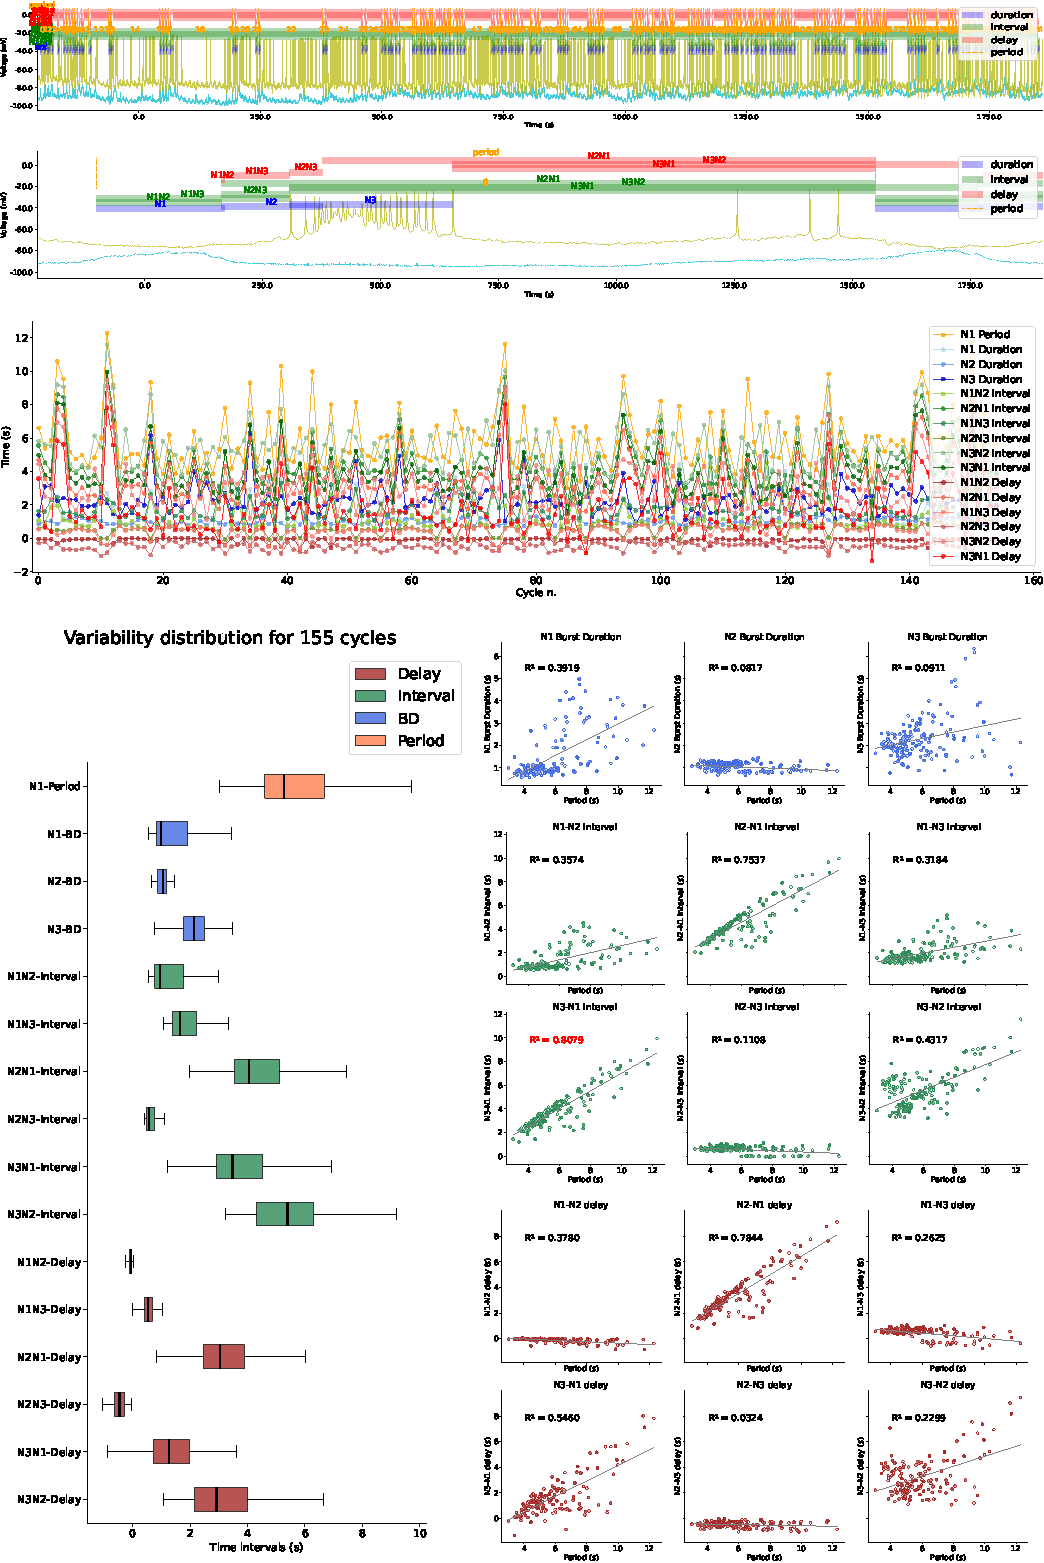
\includegraphics[width=0.9\textwidth]{./img/invariants/data/SUSSEX/prep1/images/3phases/panel_with_intervals.pdf}
	\caption{\textbf{Spontaneous case 3}: Panel of intervals distribution and dynamical invariants for the three phases in the CPG for spontaneous activity.}
	\label{fig:prep1 invariants}
\end{figure}


In figure \ref{fig:spontaneous pairplot comparison} there are represented the pairplots for each of these three experiments, with all possible combinations between intervals. Note that, for a better representation, there are only two phases taken here into account N1 and N3. Most part of the time-intervals representing N2 phase are contained in N1N3 delay which goes from the end of N1 to the start of N3 (see \ref{subsec:intervals}). The intervals' relations with the period correspond to the first column, the rest of them are combinations between all possible intervals, including the period defined from N3 start to N3 end. We see again that each recording has a different variability distribution, in the first panel there are robust dynamical invariants, also between intervals. In the second panel can be appreciated that there are still o strong linear correlations for any interval but a distribution between N1 and N3, it is interesting to see that the N1-BD has a really strong linear relation with N1N3 interval which suggest all variability in that phase comes from the burst duration, and the N2 phase was mostly constant. In the last panel we can appreciate this increase in the correlation between N1-BD and the period and the decrease in the correlation with the N3-BD, this is shown in the linear correlation unveiled in this pairplot by the N3N1-Interval and N3N1-Delay, representing the constancy in the time duration of the burst.  

\begin{figure}[htbp]
	\centering
	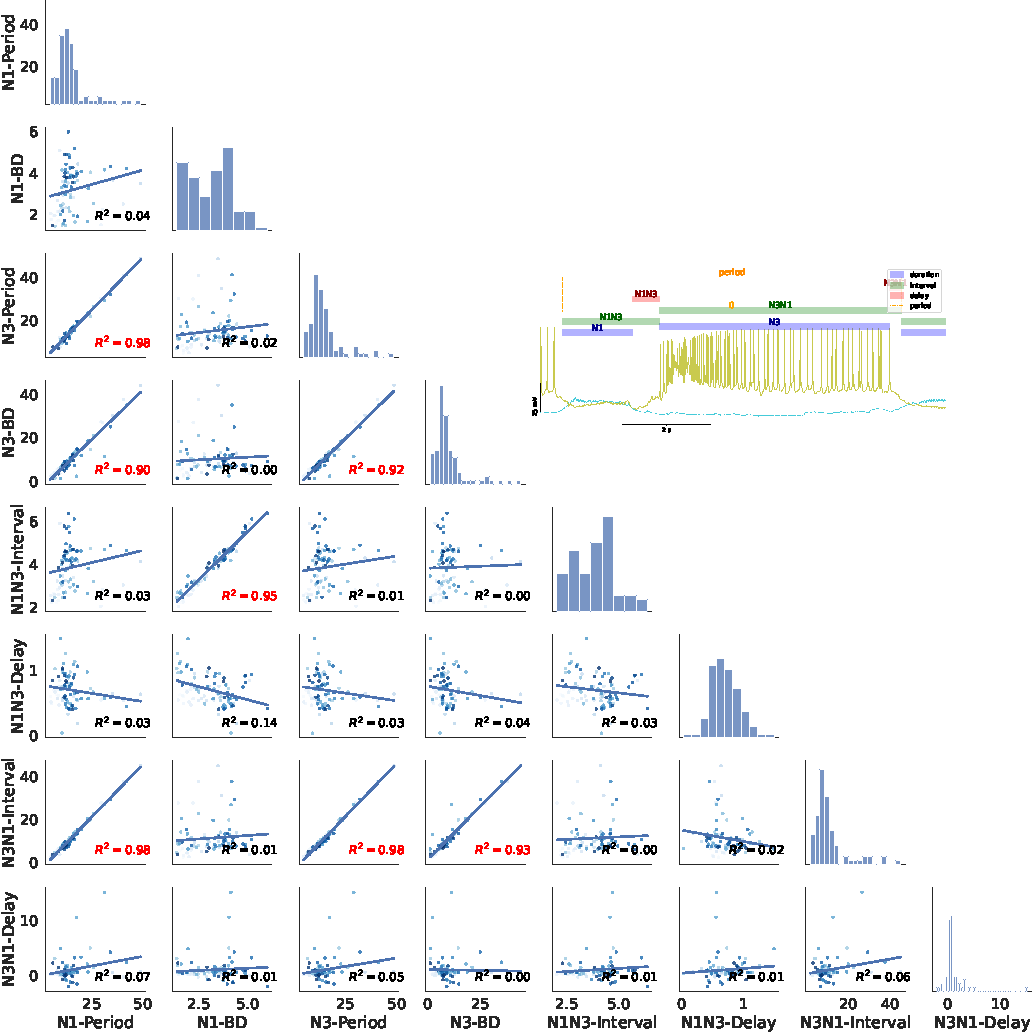
\includegraphics[width=0.48\textwidth]{./img/invariants/data/SUSSEX/prep2/images/2phases/panel_with_pairplot.pdf}
	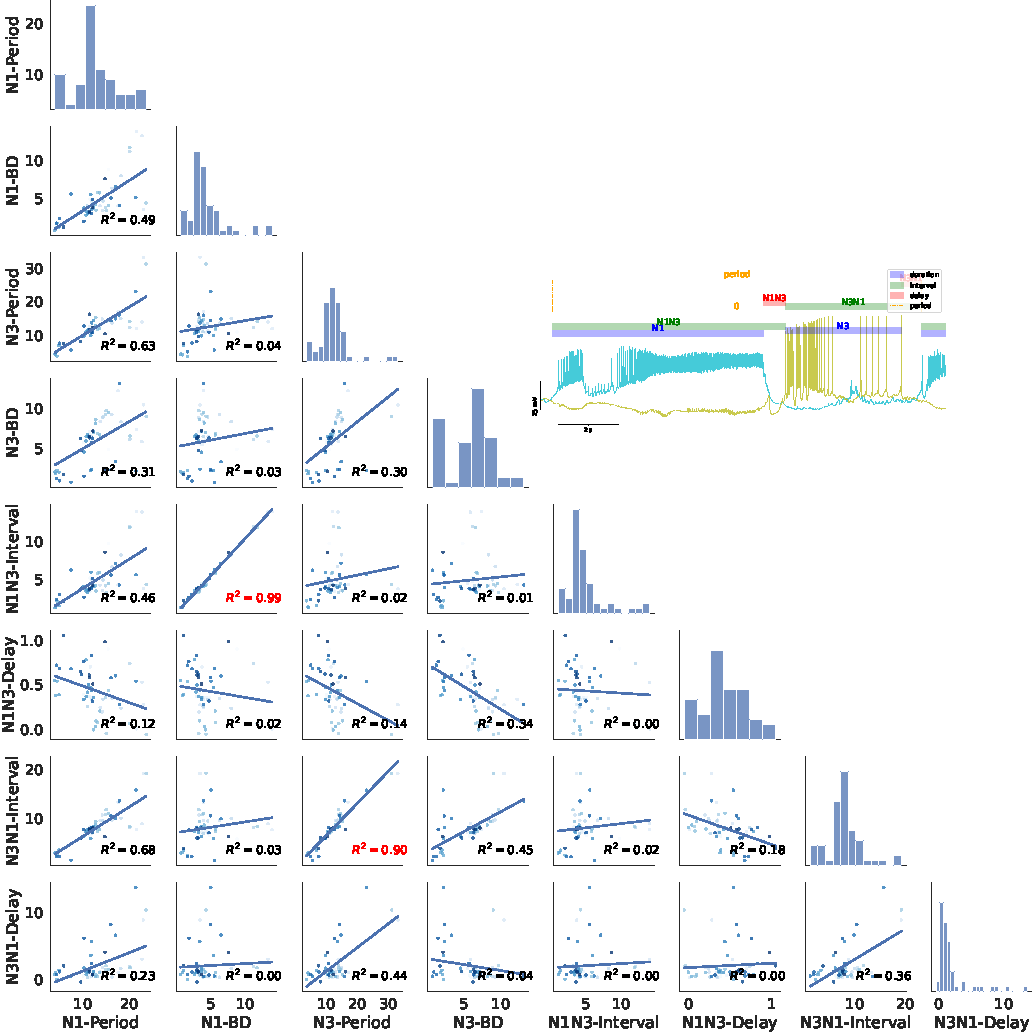
\includegraphics[width=0.48\textwidth]{./img/invariants/data/SUSSEX/prep3/images/2phases/panel_with_pairplot.pdf}
	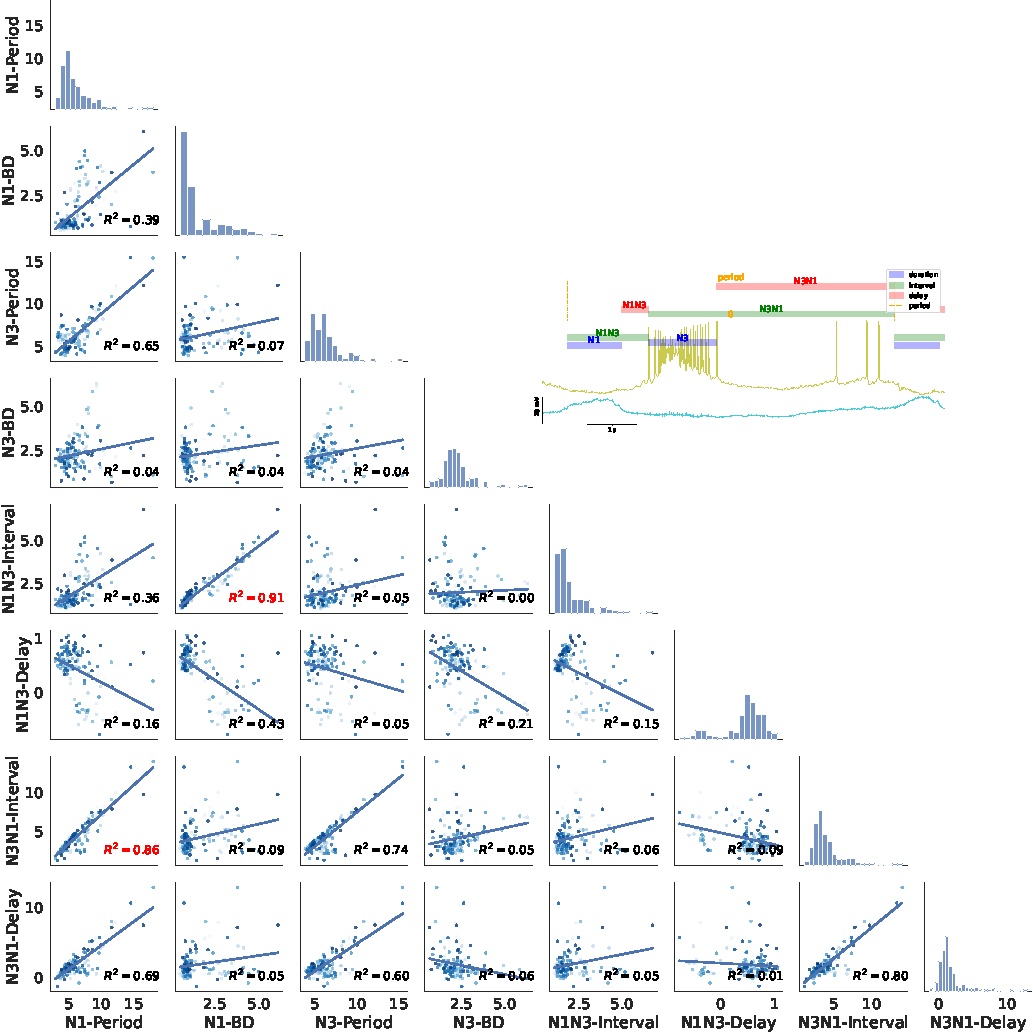
\includegraphics[width=0.48\textwidth]{./img/invariants/data/SUSSEX/prep1/images/2phases/panel_with_pairplot.pdf}
	\caption{Panel of the pairplots for all possible combinations between the time intervals for two phases (N1 and N3) in the CPG recordings for the three examples of spontaneous activity recordings.}
	\label{fig:spontaneous pairplot comparison}
\end{figure}


%\clearpage
%\newpage
\subsection{Invariants in SO driven activity}
As we saw before, SO role in the feeding CPG is modulatory, which means, that modifies the rhythm once it is activated. In the model analysis, in section \ref{subsec:so driven} we showed that when the variability in the simulations was induced by adding a ramp current in SO neuron, the time-intervals variability was distributed between N1 and N3 phases, having both a strong correlation with the period, increasing the $R^2$ values. Therefore, in the living recordings we can expect that the variability cycle-by-cycle is distributed during the modulation of SO, which is connected to N1M and N3t (see Fig. \ref{fig:feeding distribution}). 

In this subsection we will see an example from a spontaneous activity that for two lapses of time during te recording the SO was modulating. This can be identified by the inhibition of B4 and activation of B3, in Fig. \ref{fig:SO-spontaneous-driven} this process is represented in the original data. In that figure it can also be seen how during the SO modulation, the rhythm is "stabilized" with less variability in the intervals duration. The characterization of the variability of the time intervals and their relation to the cycle period for this trace is depicted in Figs \ref{fig:so spontaneous invariants 1},\ref{fig:no so spontaneous invariants} and \ref{fig:so spontaneous invariants 2}, when SO is modulating, when it ceases its modulation and when it then restarts it, respectively. 


 \begin{figure}[htbp]
 	\centering
 	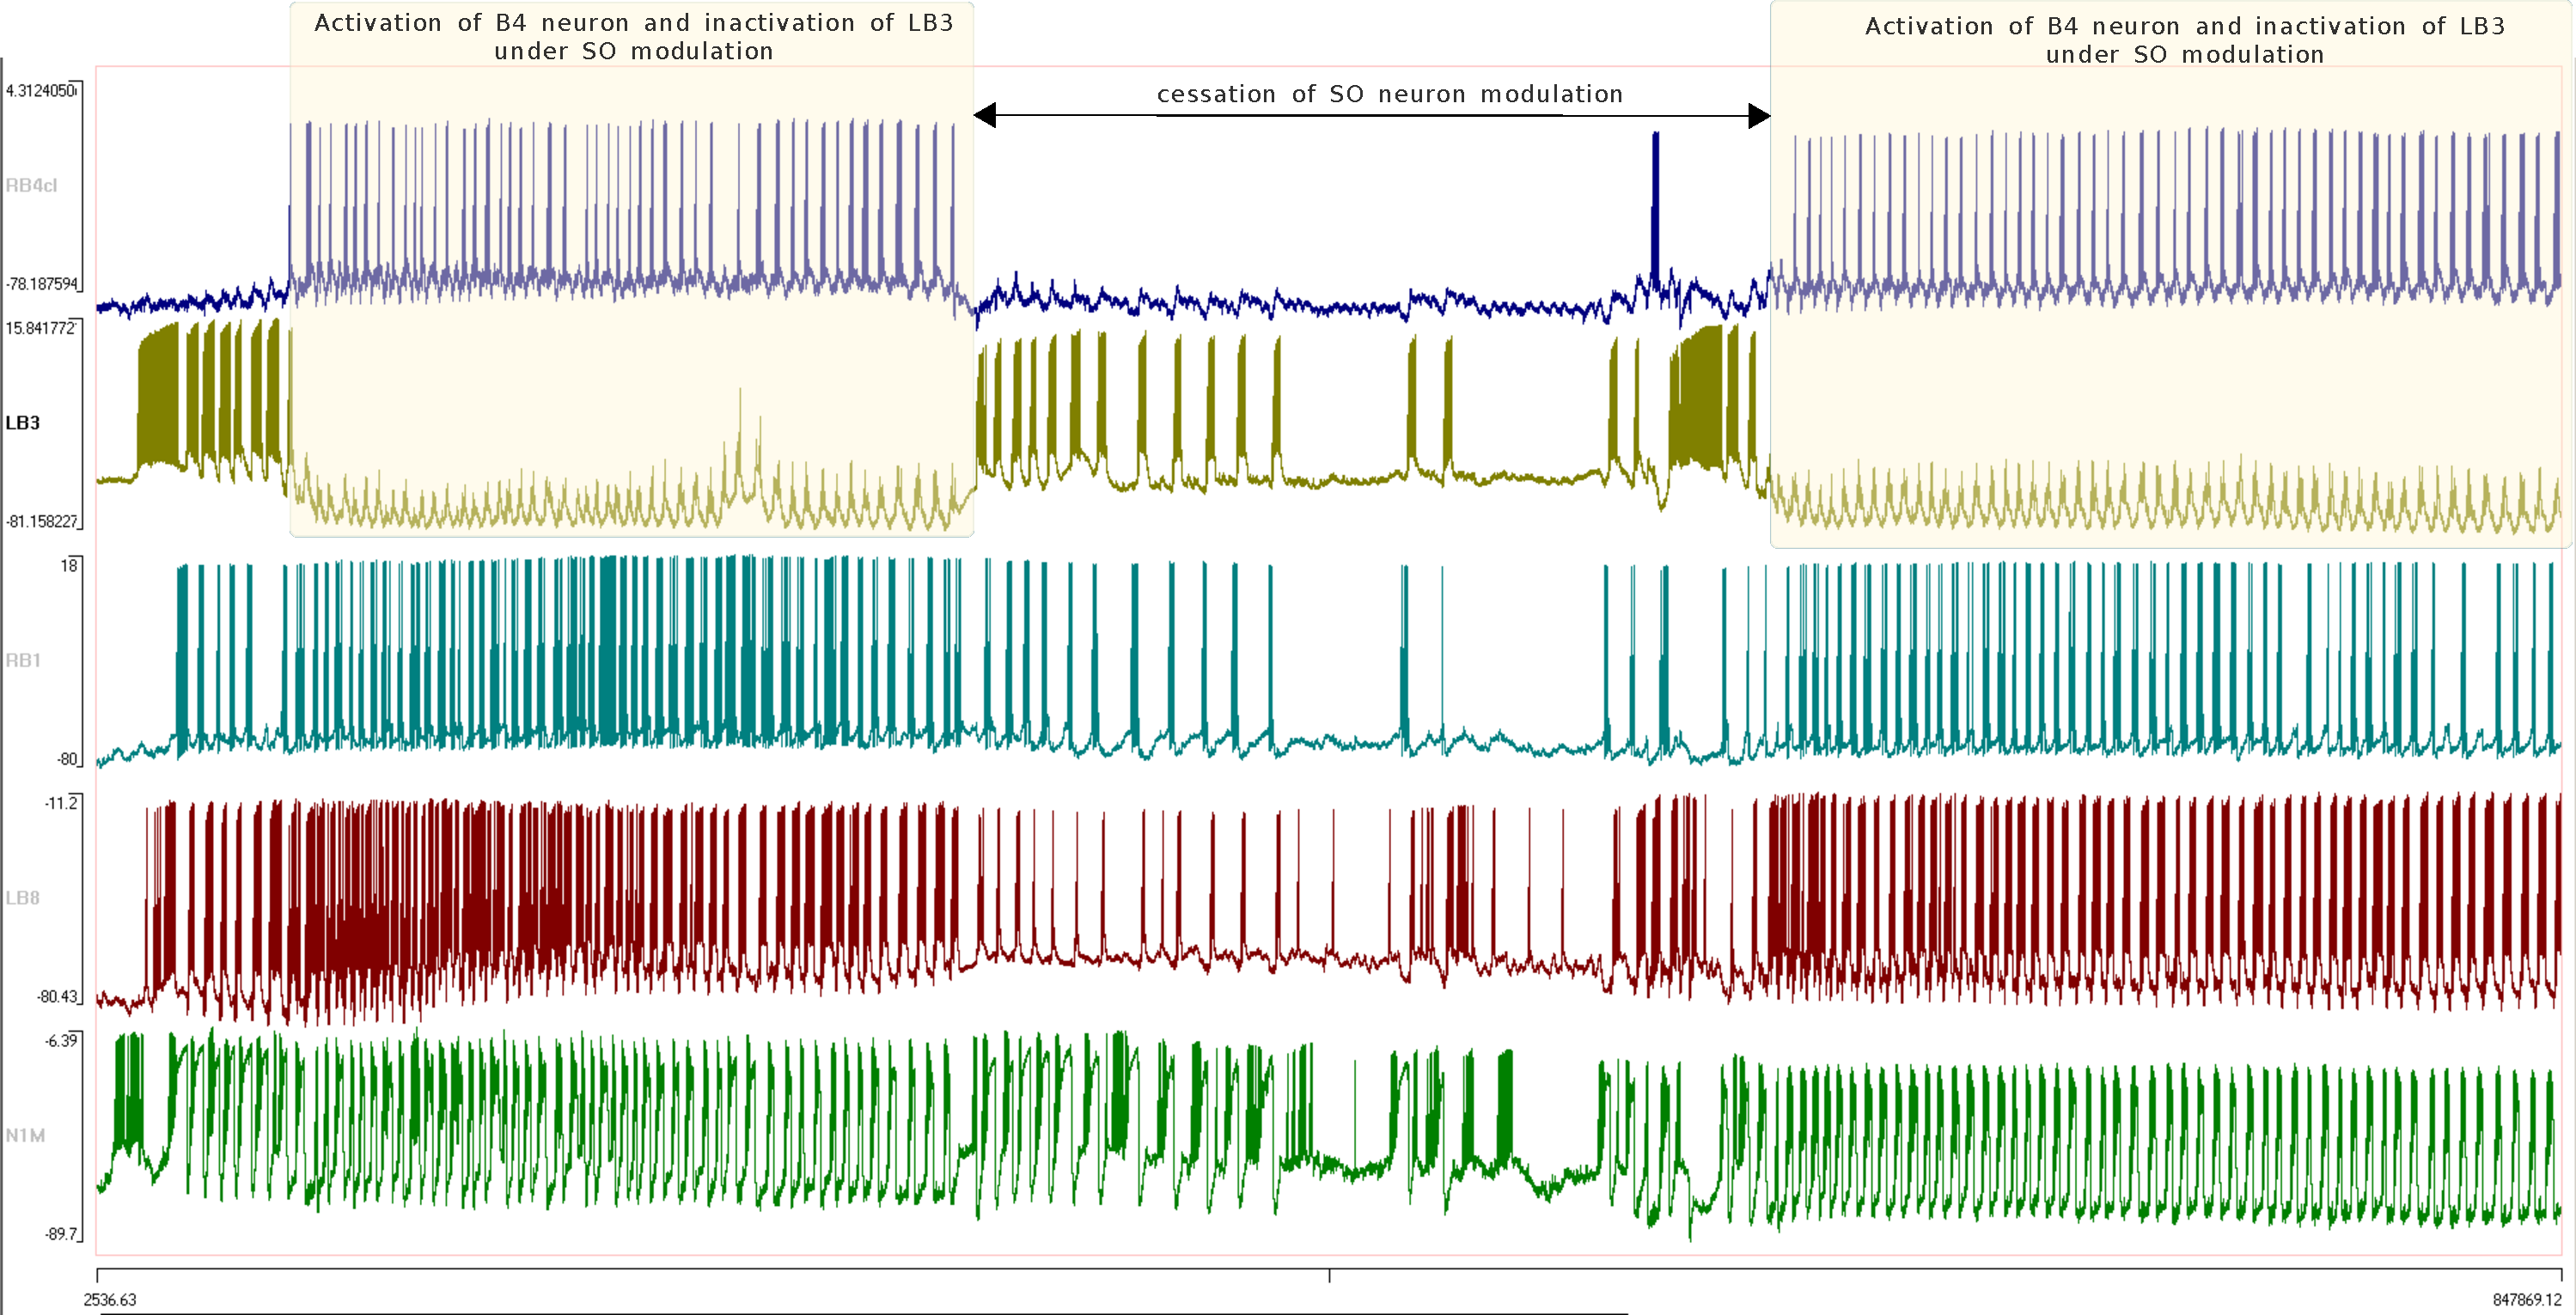
\includegraphics[width=\textwidth]{./img/invariants/SO-spontaneuous-driven.pdf}
 	\caption{Representation of the spontaneous recording with lapses of SO modulation. The parts of the recording with yellow background the activity was modulated by SO. From top to bottom, intracellular recording of a neuron from the B4 cluster, B3 motoneuron, B1 motoneuron, B8 motoneuron, N1M interneuron}
 	\label{fig:SO-spontaneous-driven}
 \end{figure}

While the rhythm is driven in SO we see how the variability for N1-BD and N3-BD is contained, represented in the boxplots of Figs. \ref{fig:so spontaneous invariants 1} and \ref{fig:so spontaneous invariants 2}, and also in the third panel representing the duration of each interval per cycle. In the correlation of the intervals with the period, although $R^2$ value is not significantly high, N1-BD and N3-BD have around 0.7 and 0.3 in both cases, pointing to this redistribution of the variability, since this is shifted in the period of time while SO stops its modulation. In Fig. \ref{fig:no so spontaneous invariants} the $R^2$ value of N1-BD is in the order of 0.9, while the N3-BD not only low but close to 0. Although this example had only a few cycles, this suggest that the variability in that lapse of time was all carried by the N1 phase. In the rest of the time-intervals in the cycle, this is extrapolated, being N3N1 interval the one with the largest variability and $R^2$, since it contains N1-BD. Also, when activity ceases the N3N1 delay variability rises, which is notable compared to the rest of the experiments and the model, and might be caused by the burst shape and how the intervals where defined (see Fig. \ref{fig:no so spontaneous invariants}, first panel). This result, also matches the experimental work by \cite{elliott_temporal_1991}, that showed this distribution between N1-BD and N3-BD. In that work the SO modulation was induced by stimulating SO neuron, in Fig. \ref{fig:so induced driven invariants} there is an example inducing the SO modulation by its electrical stimulation. Again, we can see the same variability distribution between N1 and N3 phases, having N1 a strongest correlation with the period, reaching the a $R^2$ 0.8 this time. It is also important to highlight that the intervals associated to N2 phase (N1N3 delay and N3N1 delay) do not have any relation with the period, and their variability is minimal. To further compare this two panels, the pairplots for one example of spontaneous activity and the SO induced modulation are in Fig. \ref{fig:so pairplot comparison}. In the pairplot we see the same interval relations and also another strong relation between N1N3 Interval and N1-BD, that appears in both cases and supports the N1 variability and the constancy of N2phase, since in N1N3 interval, all the variability is associated with N1-BD. 

%Acabar comparación con el otro. 
 
\begin{figure}[htbp]
	\centering
	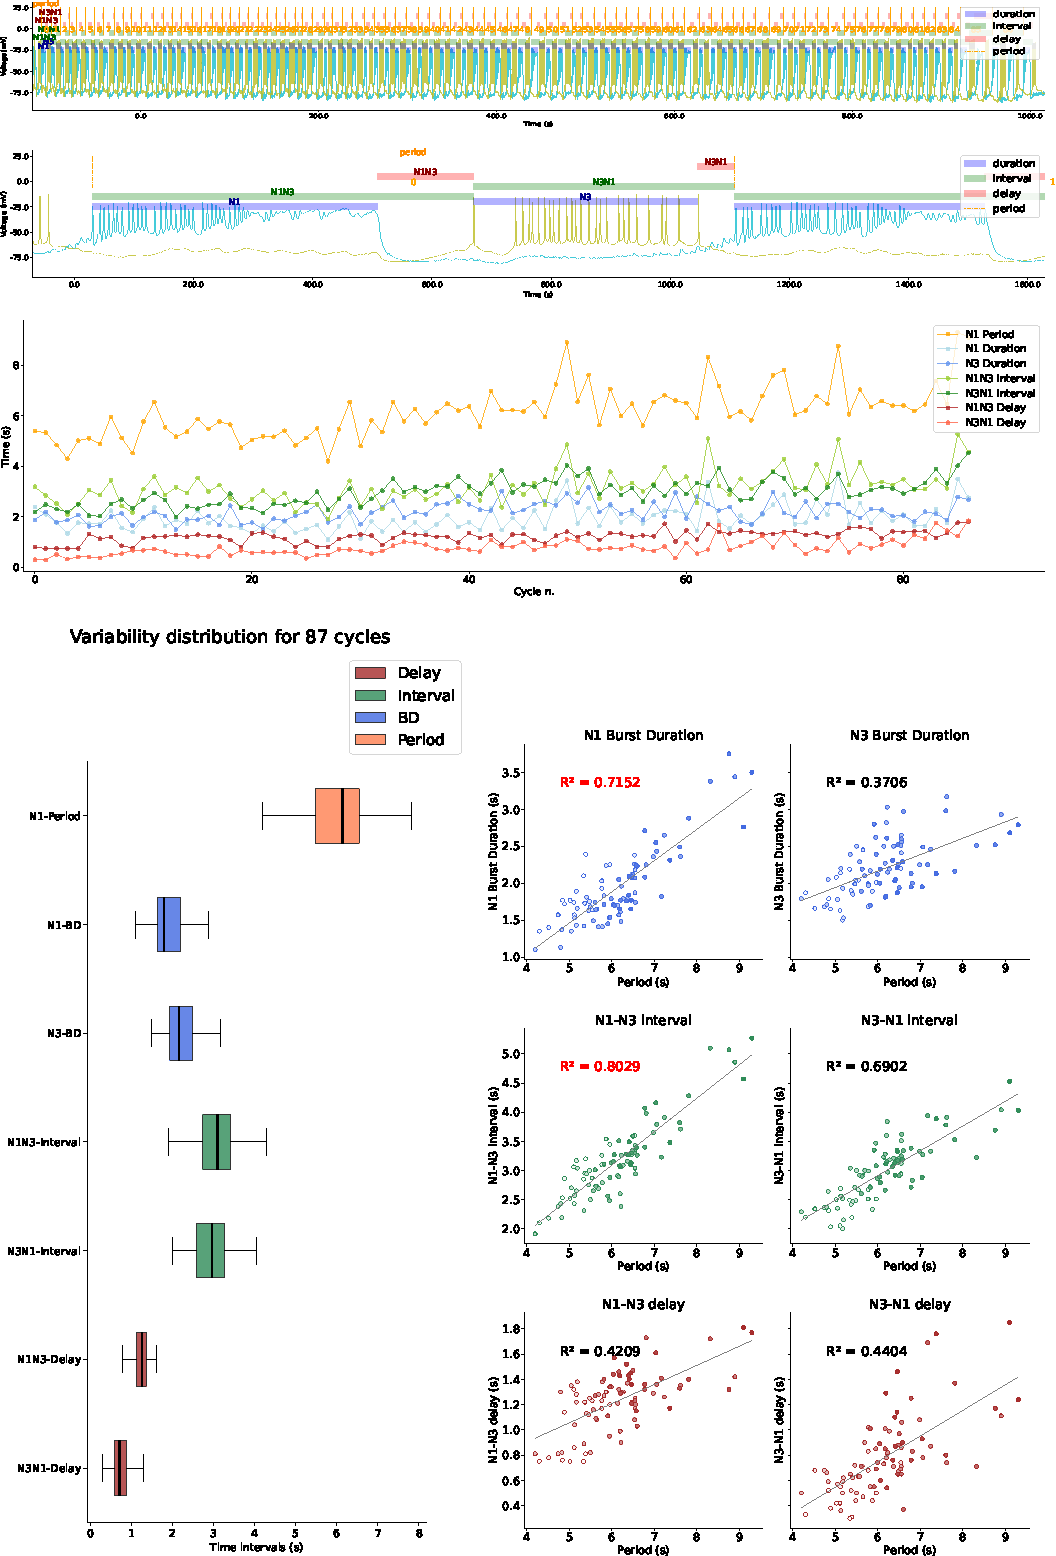
\includegraphics[width=0.95\textwidth]{./img/invariants/data/SUSSEX/prep4_so_driven_2/images/panel_with_intervals.pdf}
	\caption{\textbf{Spontaneous SO neuron driven}: Panel of intervals distribution and dynamical invariants for the two phases in the CPG for spontaneous activity driven by SO neuron.}
	\label{fig:so spontaneous invariants 2}
\end{figure}


\begin{figure}[htbp]
	\centering
	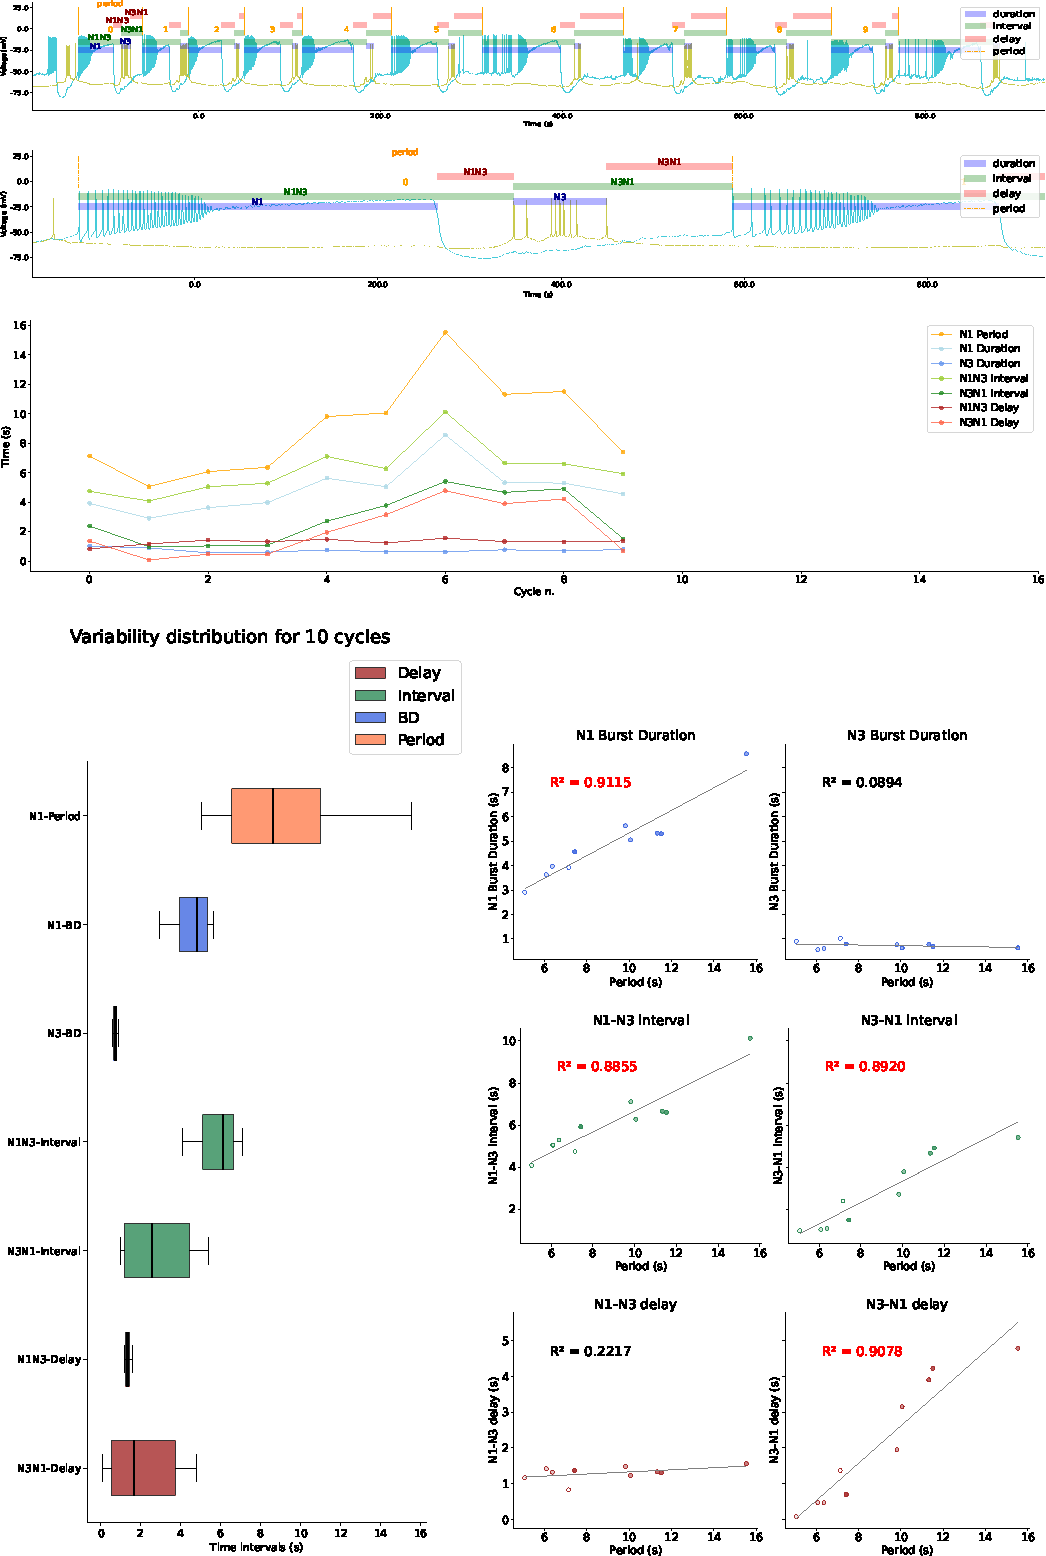
\includegraphics[width=0.95\textwidth]{./img/invariants/data/SUSSEX/prep4_so_no_driven/images/panel_with_intervals.pdf}
	\caption{\textbf{Spontaneous activity when SO-driven ceases}: Panel of intervals distribution and dynamical invariants for the three phases in the CPG for spontaneous activity.}
	\label{fig:no so spontaneous invariants}
\end{figure}
 

\begin{figure}[htbp]
	\centering
	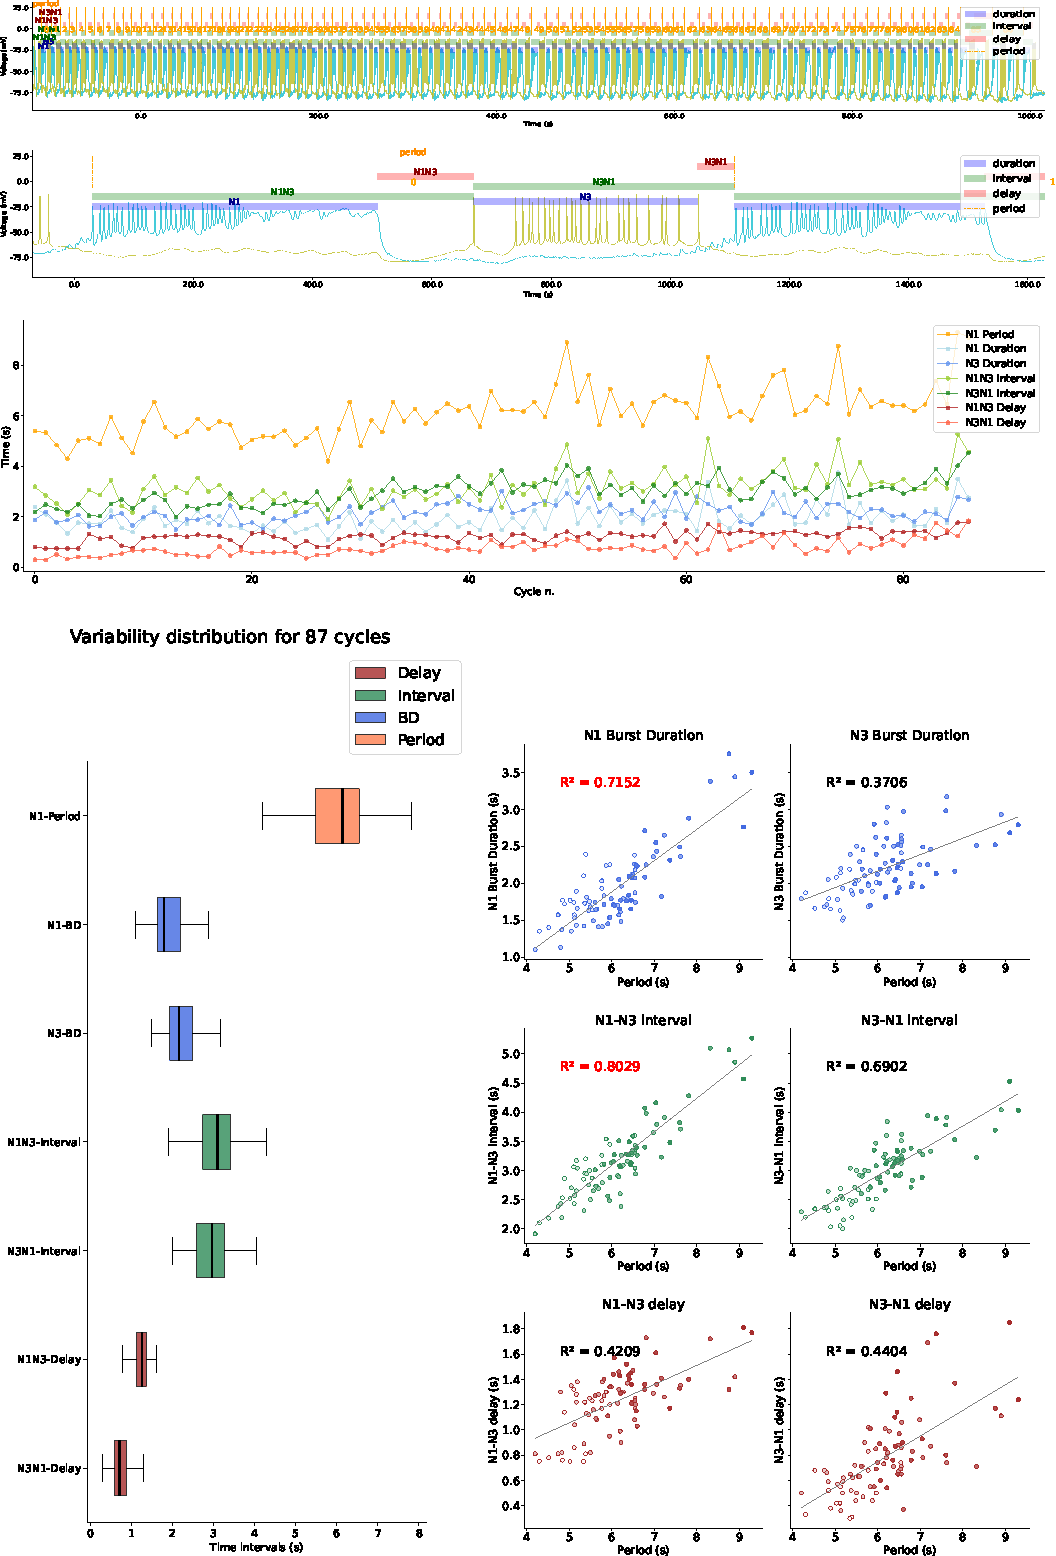
\includegraphics[width=0.95\textwidth]{./img/invariants/data/SUSSEX/prep4_so_driven_2/images/panel_with_intervals.pdf}
	\caption{\textbf{Spontaneous SO neuron modulation restarts}: Panel of intervals distribution and dynamical invariants for the two phases in the CPG for spontaneous activity driven by SO neuron.}
	\label{fig:so spontaneous invariants 1}
\end{figure}


\begin{figure}[htbp]
	\centering
	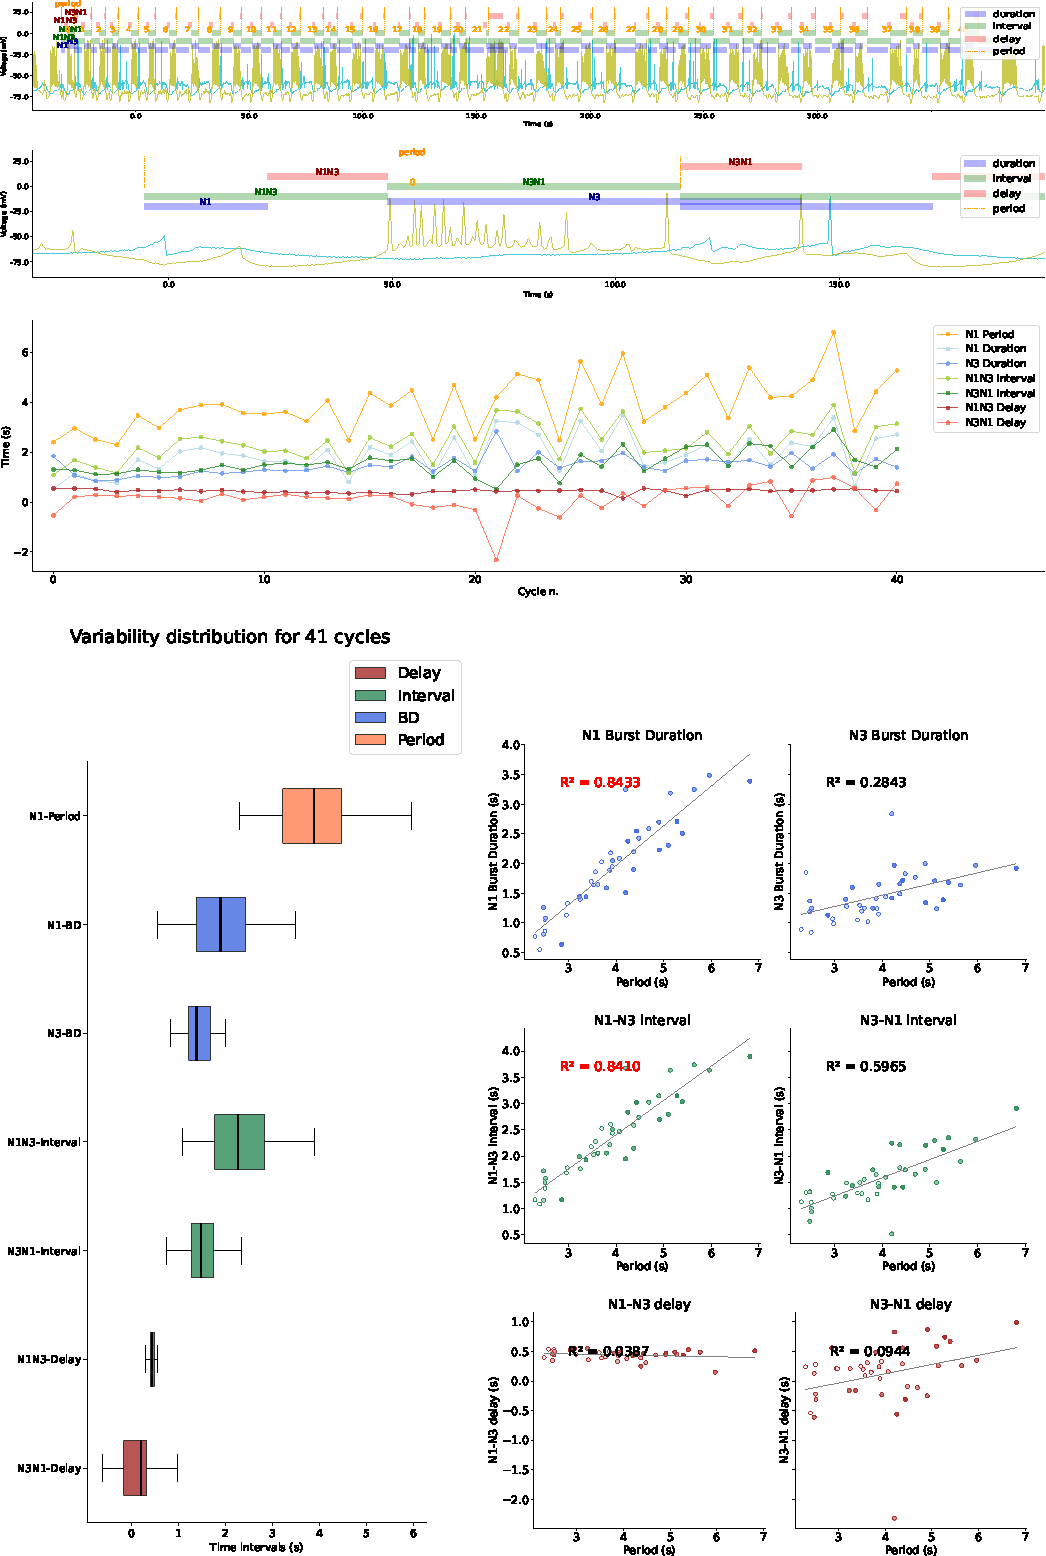
\includegraphics[width=0.95\textwidth]{./img/invariants/data/SUSSEX/SO_driven/images/panel_with_intervals.pdf}
	\caption{\textbf{Induced SO neuron modulation}: Panel of intervals distribution and dynamical invariants for the two phases in the CPG for activity driven by SO neuron induced by its electrical stimulation.}
	\label{fig:so induced invariants}
\end{figure}

 
\begin{figure}[htbp]
	\centering
	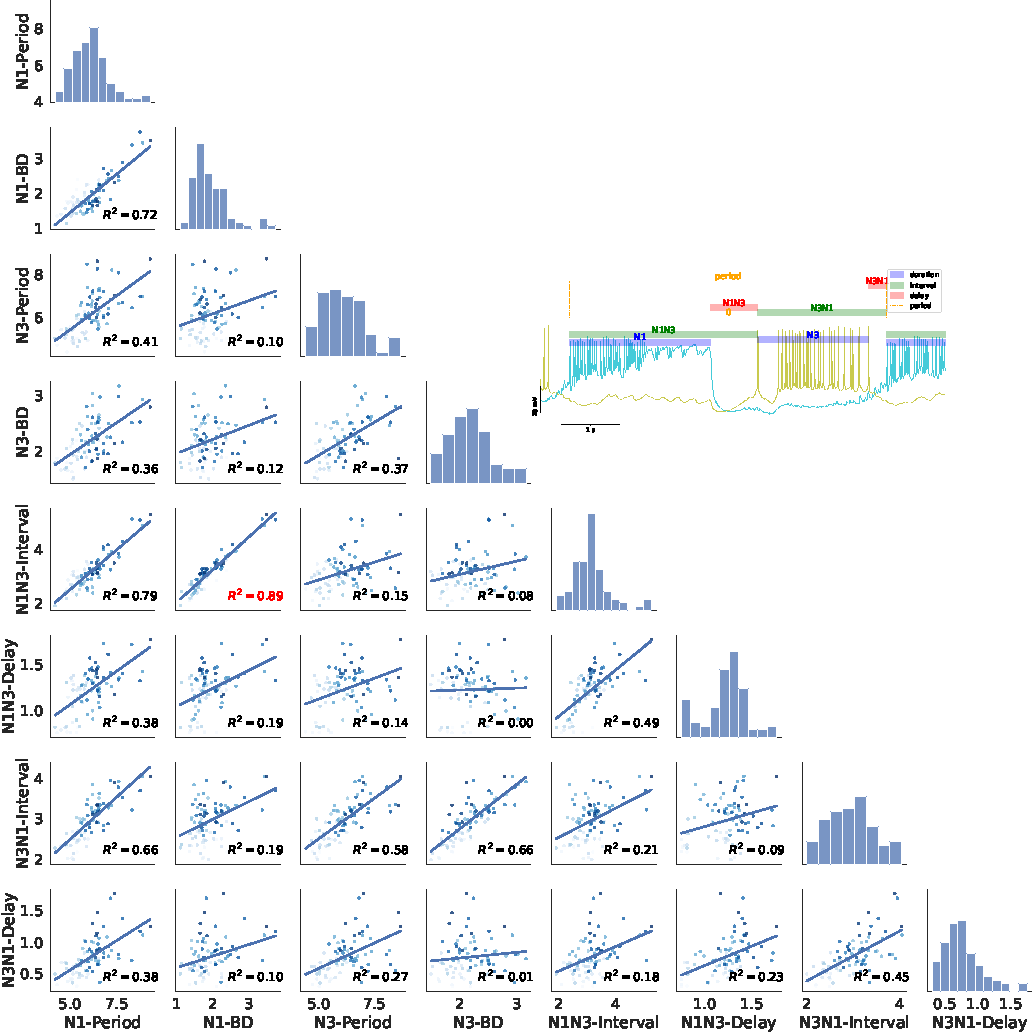
\includegraphics[width=0.48\textwidth]{./img/invariants/data/SUSSEX/prep4_so_driven_2/images/panel_with_pairplot.pdf}
	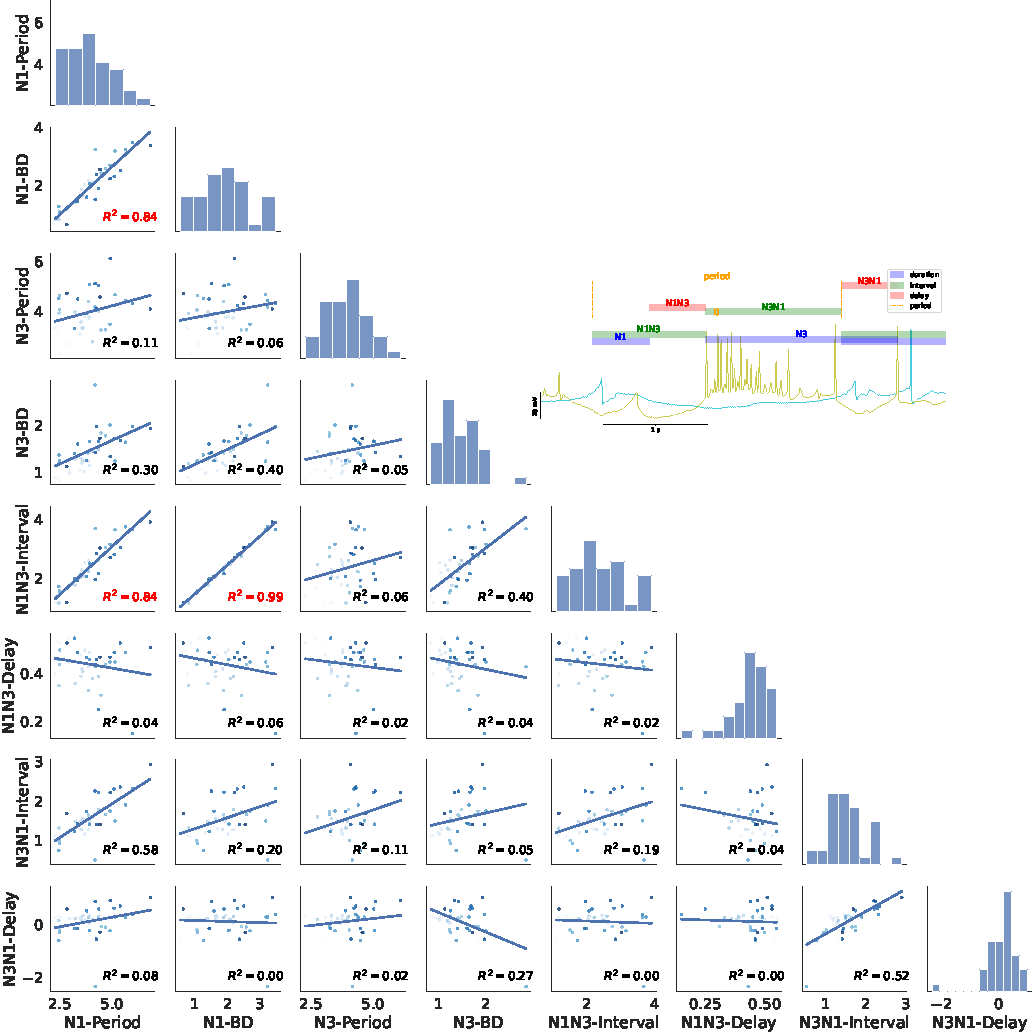
\includegraphics[width=0.48\textwidth]{./img/invariants/data/SUSSEX/SO_driven/images/panel_with_pairplot.pdf}
	\caption{Panel of the pairplots for all possible combinations between the time intervals for two phases in the CPG recordings for (left) spontaneous SO rhythm modulation and (right) the induced SO rhythm modulation}
	\label{fig:so pairplot comparison}
\end{figure}

\subsection{Invariants in MLN stimulation driven activity}
The snail's lips are connected to the cerebral ganglia by the MLN (median lip nerves). It is possible to activate CPG activity by its stimulation, simulating the initiation of the rhythm in food presence \parencite{staras_electrophysiological_2019}. This nerve directly stimulates the N1M interneuron, in charge of the initiation of the rhythm, associated to protraction phase. In Fig. \ref{fig:mln stimulation} the variability and time-intervals correlations are characterized for a recording of this induced stimulation. We can see in that figure that there is a strong linear correlation in the panel, leading the rhythm completely by N1 phase. This is visible in the robust dynamical invariant between N1 burst duration and the period and by N1N3 Interval and the period. It is also important that no other intervals have relation with the period, so both N2 and N3 phases remain constant. Note that the N1 burst duration takes a wide range of values for its duration, even at really low ranges, shorter than N3 burst for example. This is also clearly represented in the figure in the third row, where N1 burst duration and N1N3 Interval robustly follow the period. 
In Fig. \ref{fig:mln stimulation pairplot} all possible combination of time-intervals for two phases are represented. We can see there another strongly related intervals N1N3 interval with N1 burst duration, that again highlights the steadiness of N2 phase. 
This results suggest that during the MLP stimulation, the feeding rhythm variability is lead by N1 phase, activating the rhythm and stabilizing the activity. 
%Also there are some other intervals that present a tendency to a linear relation with $R^2$ close to 0.7: N3N1 Interval and N3 burst duration, and N1N3 delay and N1N3 interval 


\begin{figure}[htbp]
	\centering
	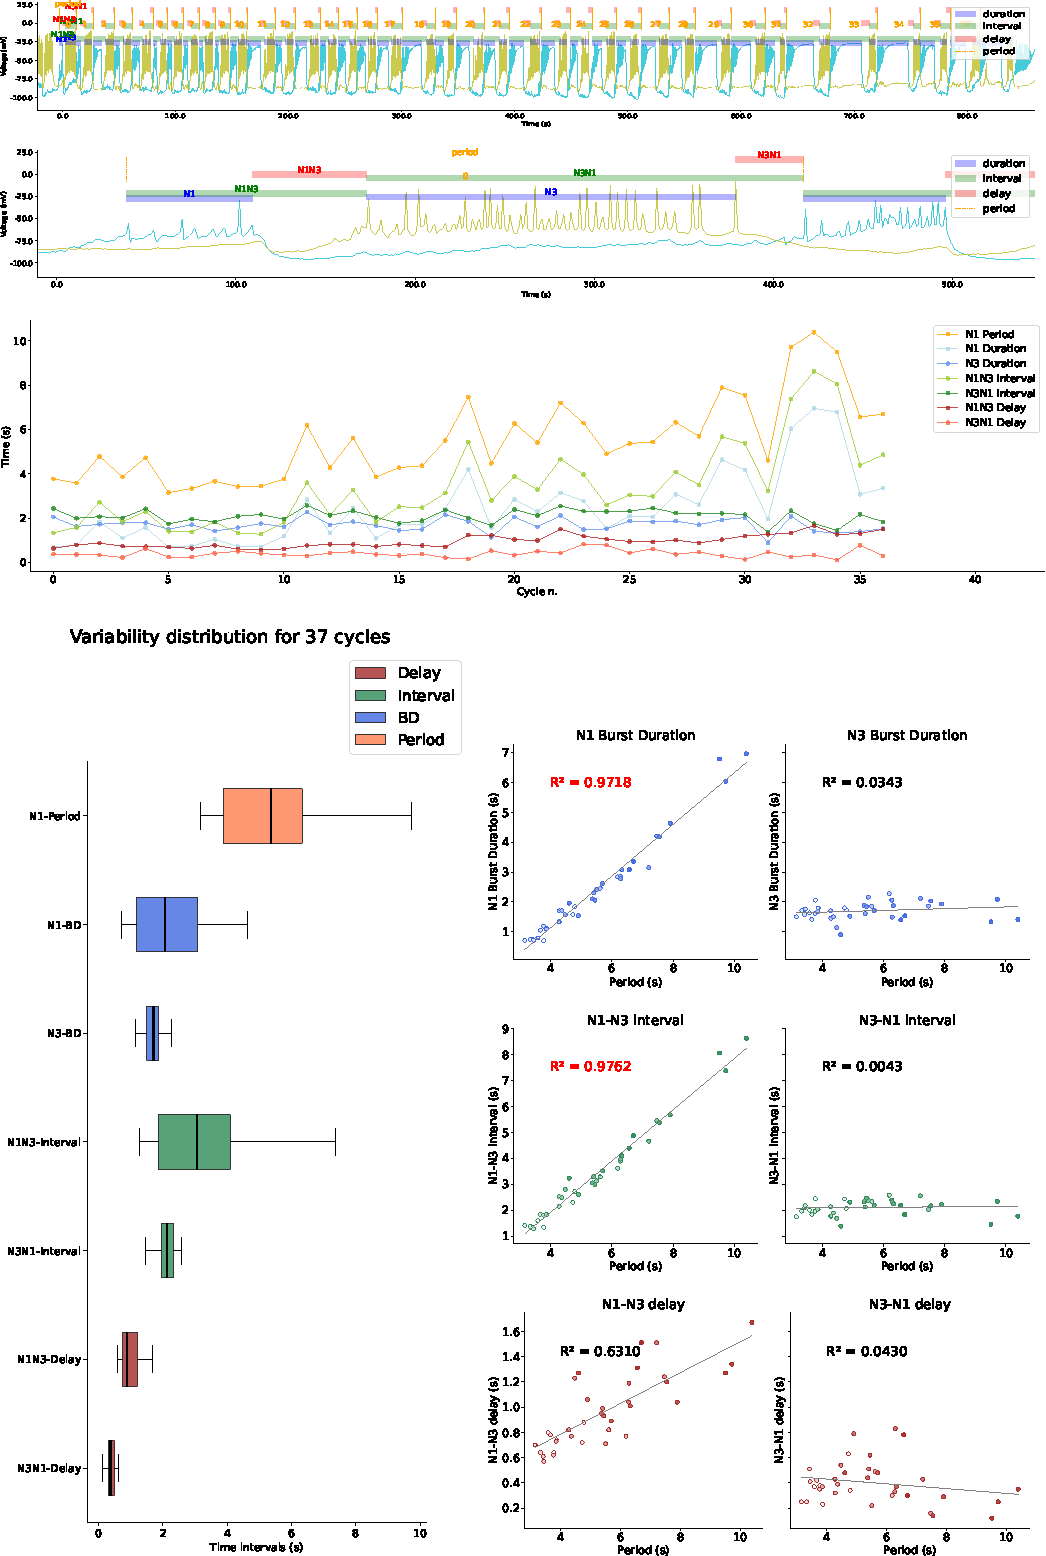
\includegraphics[width=0.9\textwidth]{./img/invariants/data/SUSSEX/MLN_driven/images/panel_with_intervals.pdf}
	\caption{\textbf{MLN stimulation}: Panel of intervals distribution and dynamical invariants for the three phases in the CPG under MLN Medium Lip Nerve (MLN) stimulation.}
	\label{fig:mln stimulation}
\end{figure}


\begin{figure}[htbp]
	\centering
	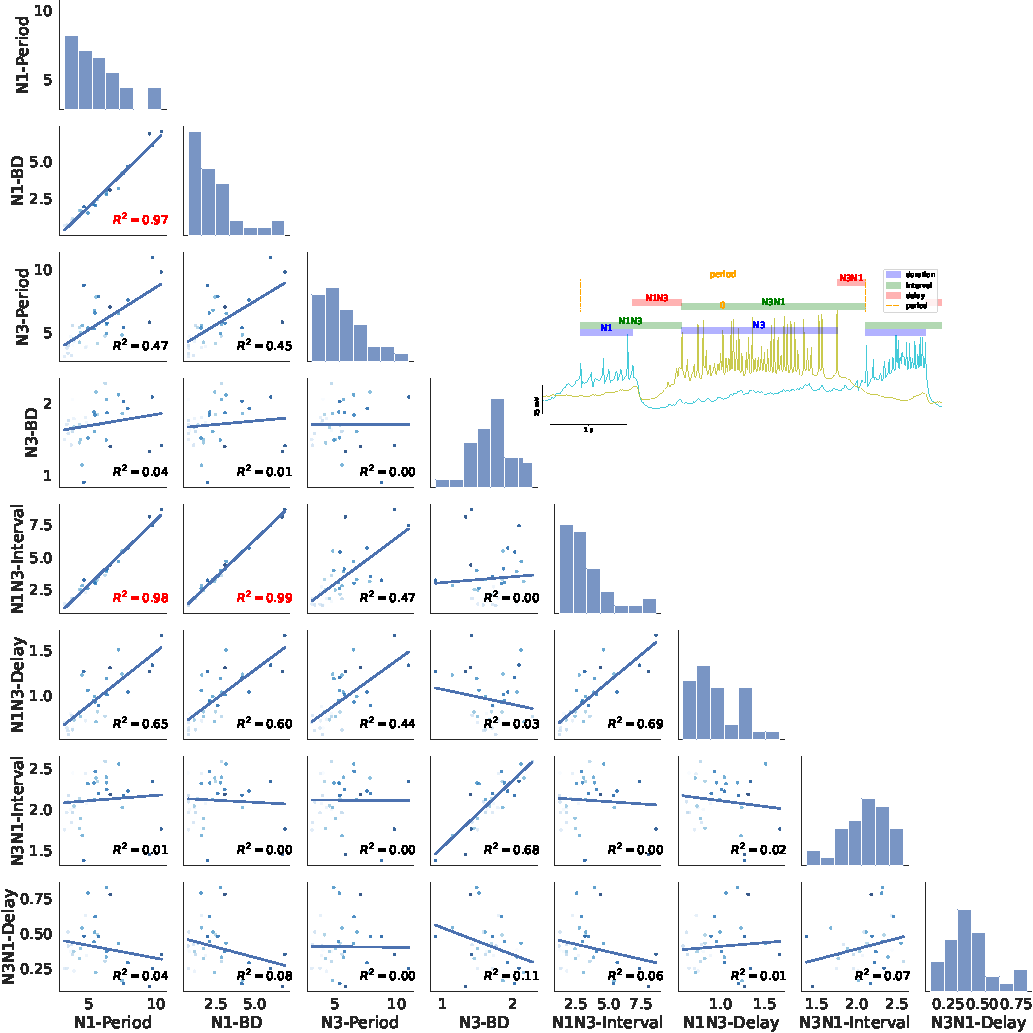
\includegraphics[width=0.9\textwidth]{./img/invariants/data/SUSSEX/MLN_driven/images/panel_with_pairplot.pdf}
	\caption{\textbf{MLN stimulation}:Pairplot of the invariants reset within cycles.}
	\label{fig:mln stimulation pairplot}
\end{figure}


\subsection{Invariants in CVa1 driven activity induced by electrical stimulation}
CV1a neuron is part of a larger population of CBIs that is influeced by sucrose, which can drive the rhythmic activity in that group of neurons. CBIs are connected by mutual excitation to interneuron N1M, involved in the rhythm initation (see Fig. \ref{fig:feeding distribution}). Therefore, it can be expected to observe in this case a stronger role of N1 phase in the variability distribution. For this case there are 4 examples of different recordings, represented from figures \ref{fig:cv1a 1 2phases} to \ref{fig:cv1a 3 2phases}. In the first three panels we can see that the stronger relation is in N1 burst duration, specially in the first case where there is a strong sequential dynamical invariant with $R^2>0.9$. The rest of the intervals conforming that sequence were not strongly related, being N3 phase more variable than the N2 phase, barely presenting variability and with no linear correlation with the period. It is interesting to highlight that not all of the cases where the variability was larger, the correlation to the period was also larger, as it is the case in example 3 in Figs. \ref{fig:cv1a 2 2phases} and \ref{fig:cv1a 4 2phases}. In those examples, the variability in N3 neuron is large but it is not related to the period. Seeing the third figure in each of those panels, we can explain it by the opposite direction of the changes in N3 (dark blue) and N1 (light blue) and the period (orange), pointing that the N3 burst is adapting to the N1 strongest variability. This distribution is maintained for the three first cases, however, in the last case this is shifted. In the example characterized in Fig. \ref{fig:cv1a 3 2phases}, the N3 burst duration has a stronger linear relation with the period than N1, presenting also a larger variability. During that period the electrode stimulating CV1a slipped away and the stimulation was not as effective as it was in the rest of the examples. We can appreciate in the correlation between N1 and the period that there are some points white-colored that correspond to the beginning of the trace, that might look as outliers but present a tendency to a linear regression.  Although this was not a methodic study, we decided to include this case since it represents the sensitivity to the circuit to changes in the context, redistributing in a flexible way the activity between the different phases, in this case from N1 to N3.

Finally, in Fig. \ref{fig:cv1a pairplot comparison} the plots for 2 phases for each panel are depicted. For some of the recordings when the N2 phase could be well identified, the pairplots for three phases are in the Appendix \ref{fig:cv1a 1 3phases pairplot},\ref{fig:cv1a 4 3phases pairplot}. In the pariplot, again we see a similar distribution in all figures except of the last one, where there are new correlations, present in the N3 burst duration with the N3N1 interval. Also there is a correlation of a negative slope in the first case, in case N3-BD and N3N1 Delay, representing a regular overlapping of N1 and N3 phases. 
%
%%and the complete map of their locations is shown in Figure 3A. https://static-content.springer.com/esm/art%3A10.1186%2F2042-1001-2-4/MediaObjects/13232_2011_20_MOESM3_ESM.jpeg
%Sucrose drives rhythmic activity in CBIs activating the feeding circuit by the conection
%\paragraph{Example 1}

\begin{figure}[htbp]
	\centering
	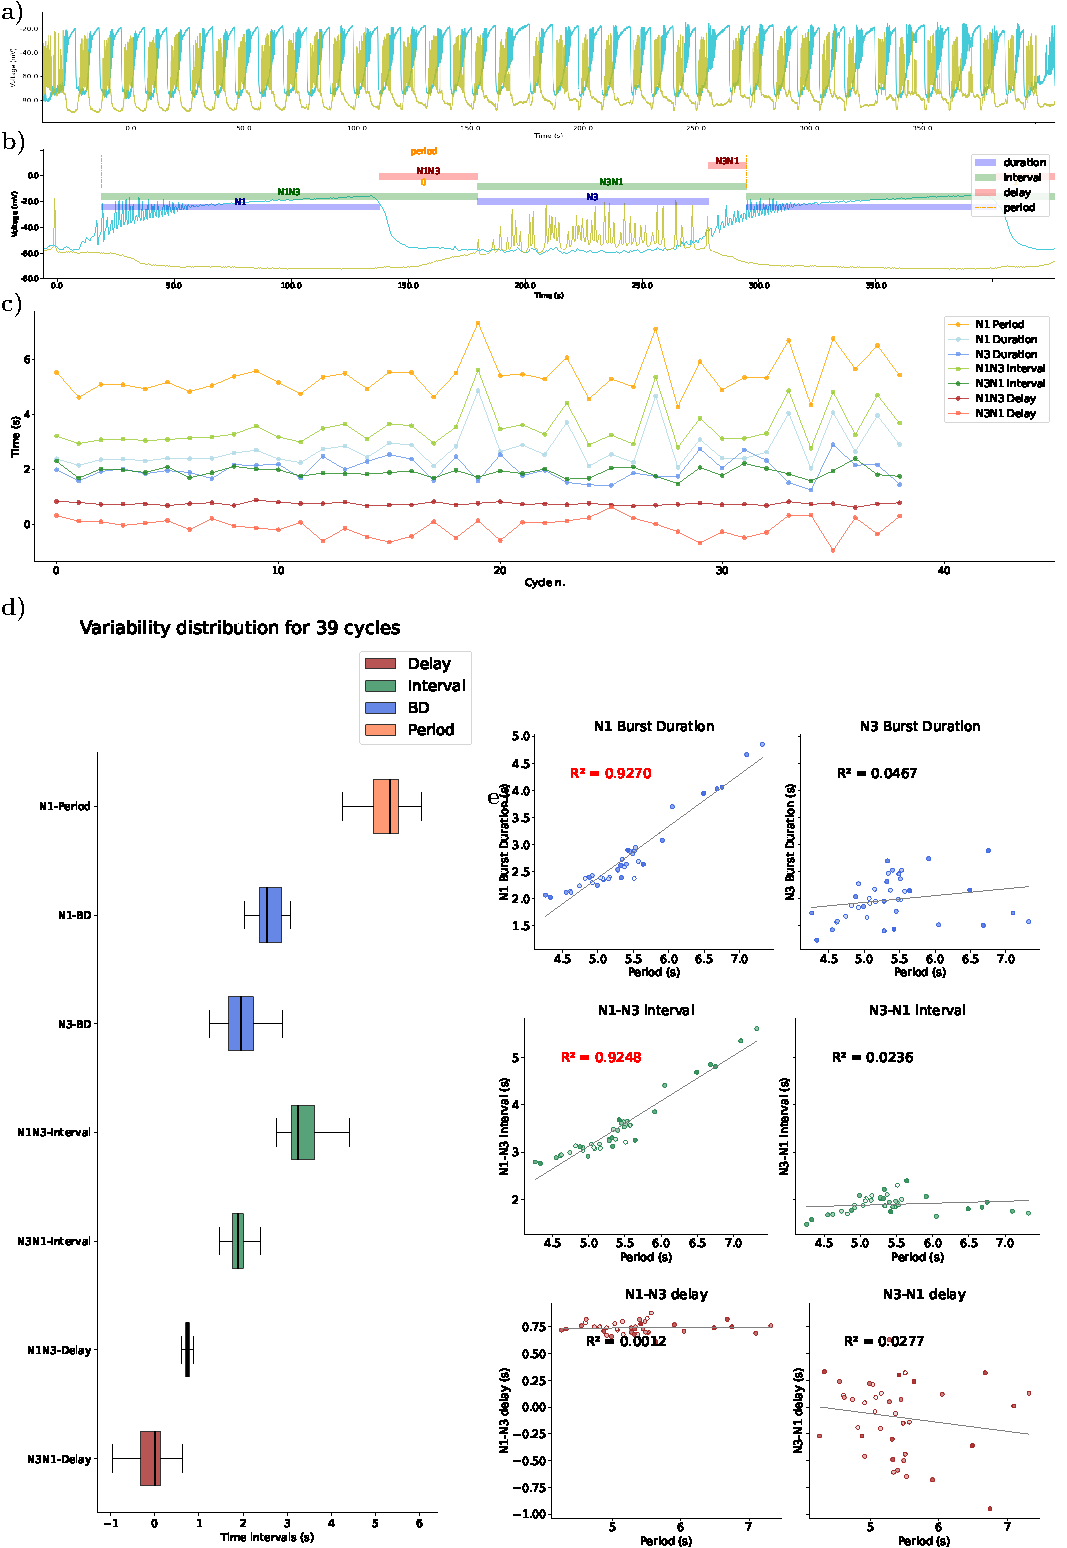
\includegraphics[width=0.9\textwidth]{./img/invariants/data/SUSSEX/CV1a_driven1/images/2phases/panel_with_intervals.pdf}
	\caption{\textbf{CV1a driven case 1}: Panel of intervals distribution and dynamical invariants for the two phases in the CPG under CV1a stimulation.}
	\label{fig:cv1a 1 2phases}
\end{figure}

%\paragraph{Example 2}


\begin{figure}[htbp]
	\centering
	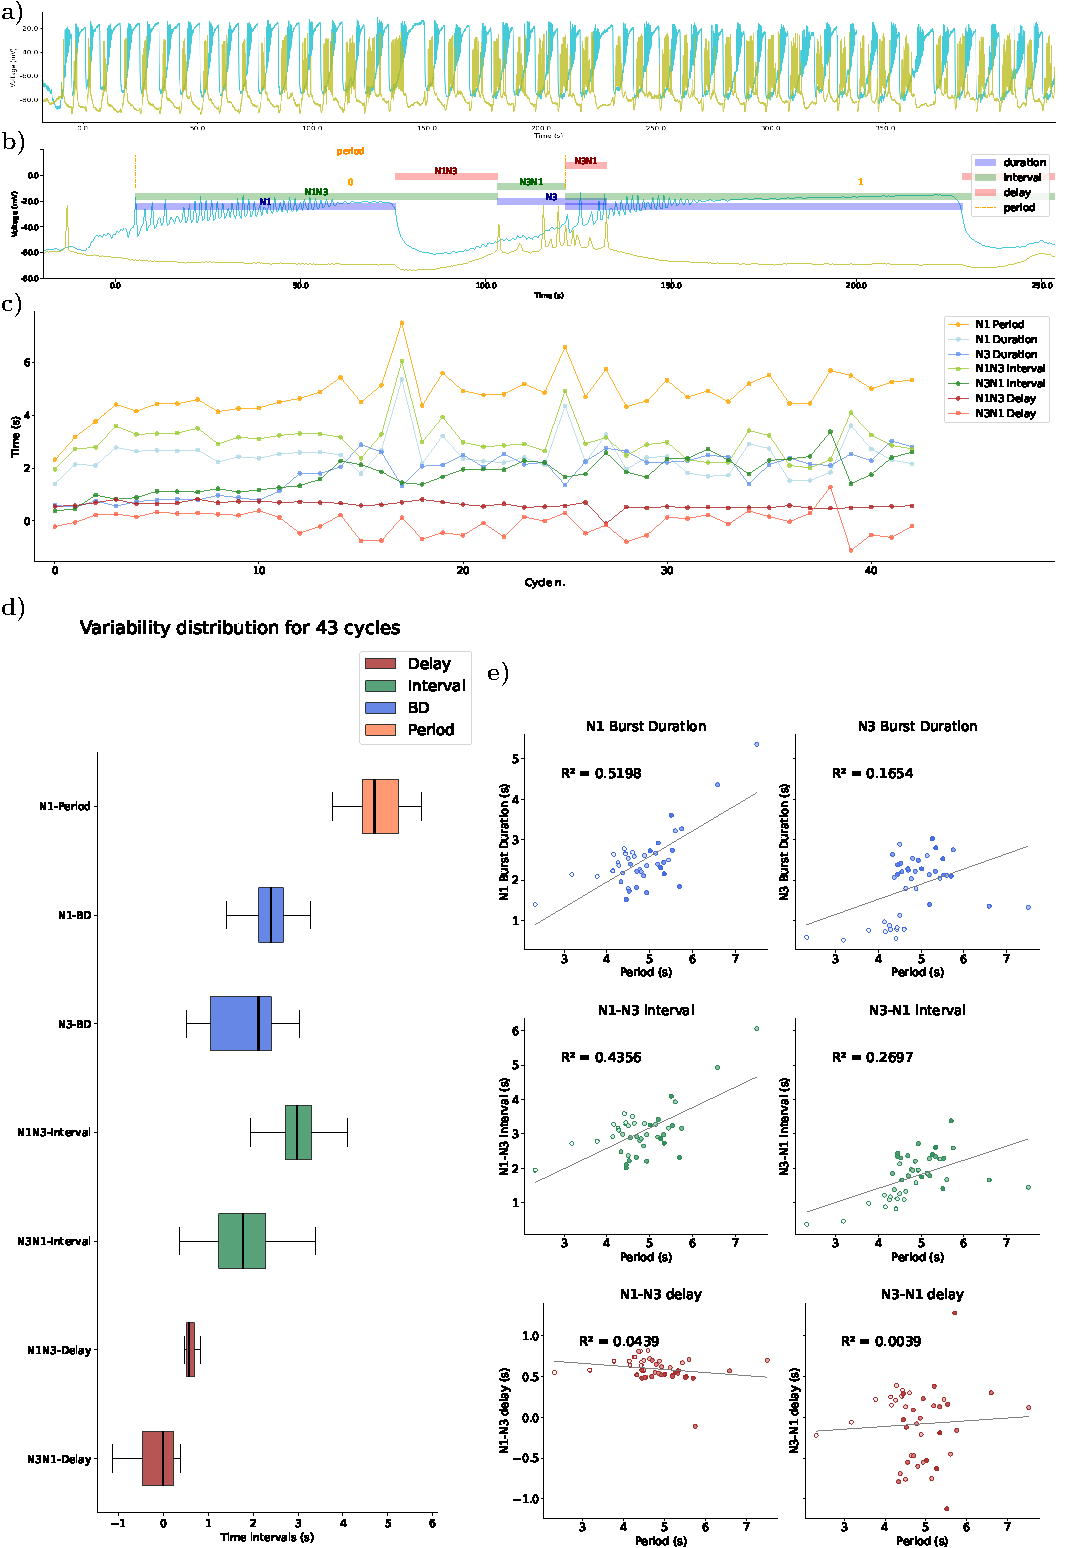
\includegraphics[width=0.9\textwidth]{./img/invariants/data/SUSSEX/CV1a_driven2/images/panel_with_intervals.pdf}
	
	\caption{\textbf{CV1a driven case 2}: Panel of intervals distribution and dynamical invariants for the two phases in the CPG under CV1a stimulation.}
	\label{fig:cv1a 2 2phases}
\end{figure}


%\paragraph{Example 4}

\begin{figure}[htbp]
	\centering
	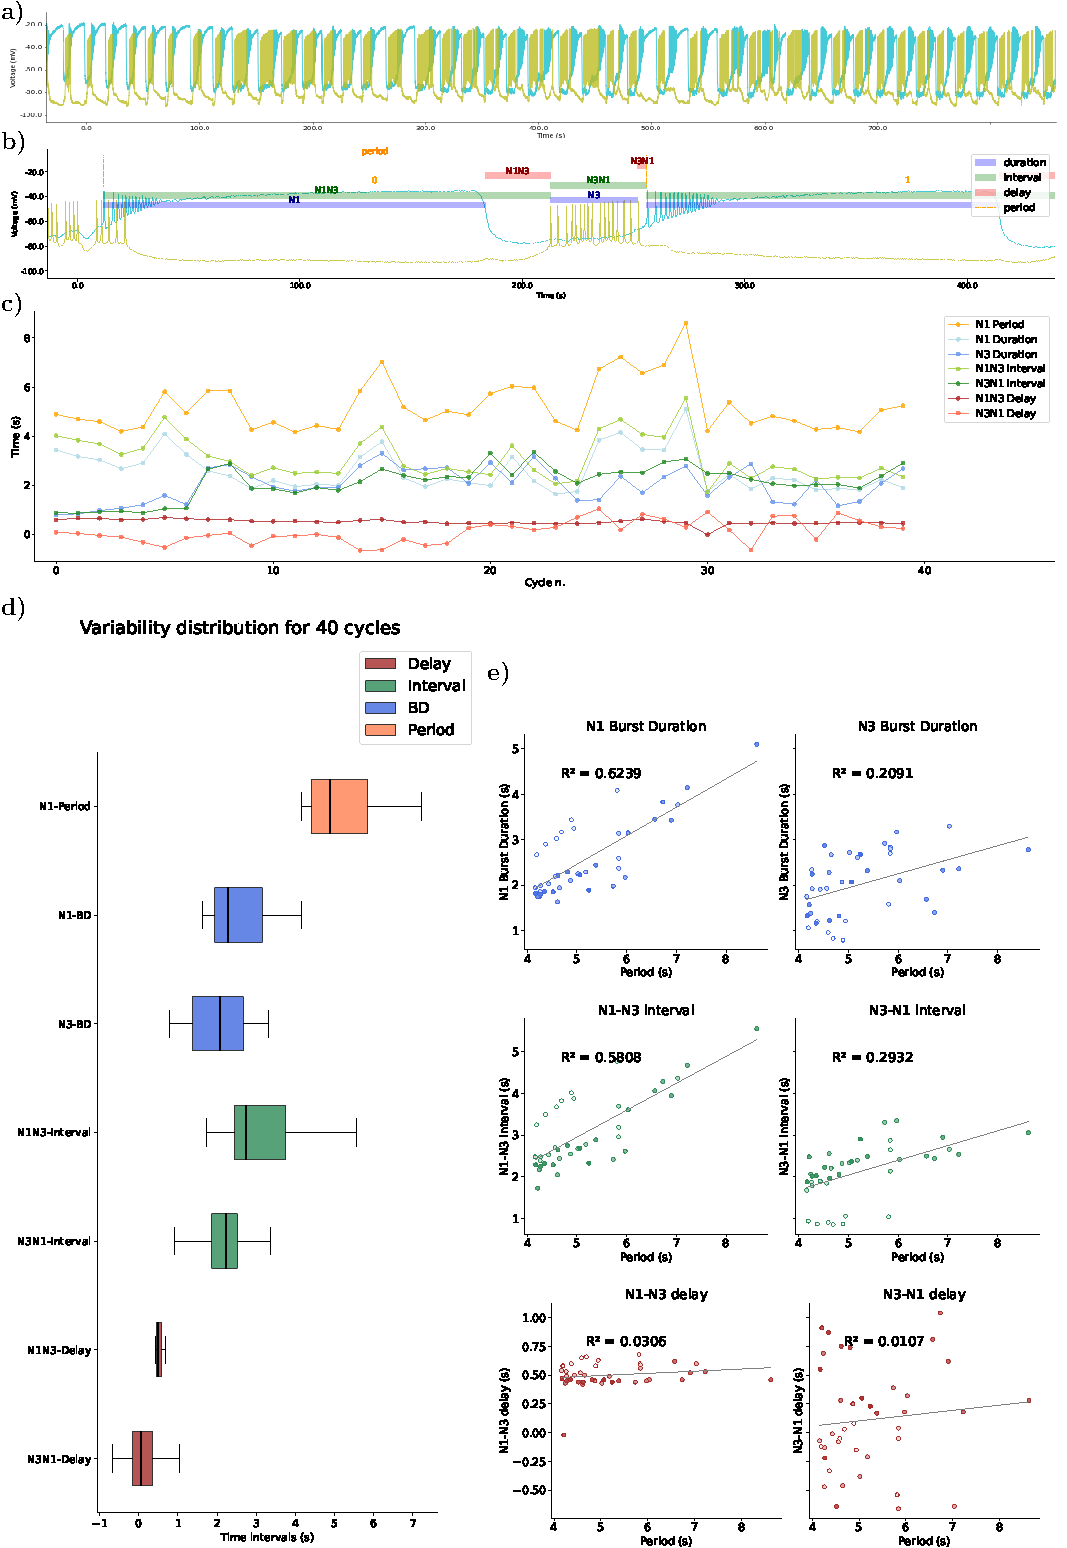
\includegraphics[width=0.9\textwidth]{./img/invariants/data/SUSSEX/CV1a_driven4/images/2phases/panel_with_intervals.pdf}
	\caption{\textbf{CV1a driven case 3}: Panel of intervals distribution and dynamical invariants for the two phases in the CPG under CV1a stimulation.}
	\label{fig:cv1a 4 2phases}
\end{figure}


%\paragraph{Example 3}


\begin{figure}[htbp]
	\centering
	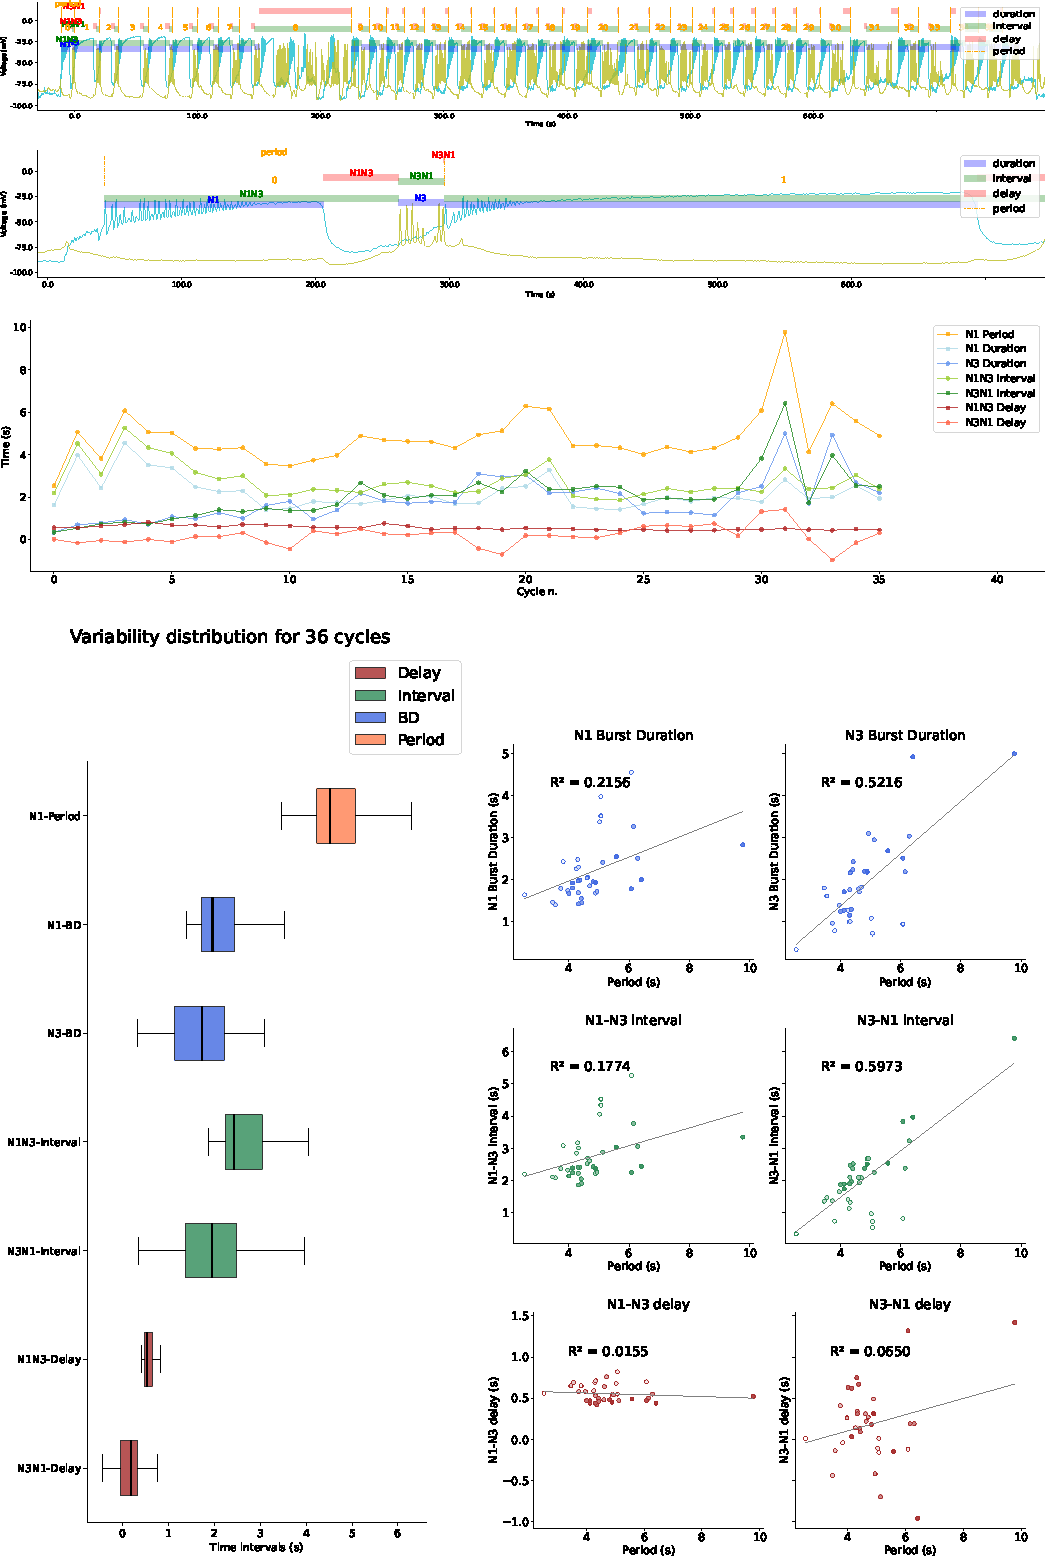
\includegraphics[width=0.9\textwidth]{./img/invariants/data/SUSSEX/CV1a_driven3/images/panel_with_intervals.pdf}
	\caption{\textbf{CV1a driven case 4}: Panel of intervals distribution and dynamical invariants for the two phases in the CPG under CV1a stimulation.}
	\label{fig:cv1a 3 2phases}
\end{figure}




\begin{figure}[htbp]
	\centering
	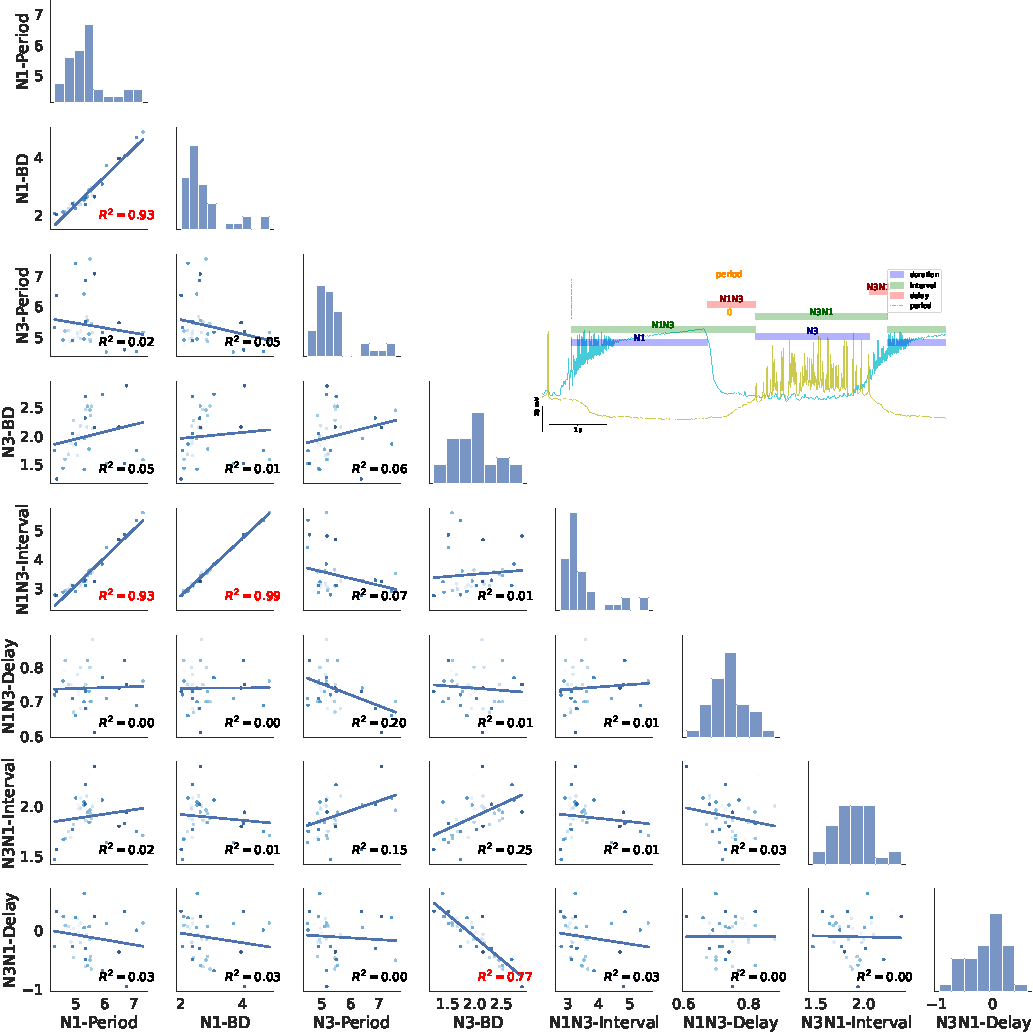
\includegraphics[width=0.48\textwidth]{./img/invariants/data/SUSSEX/CV1a_driven1/images/2phases/panel_with_pairplot.pdf}
	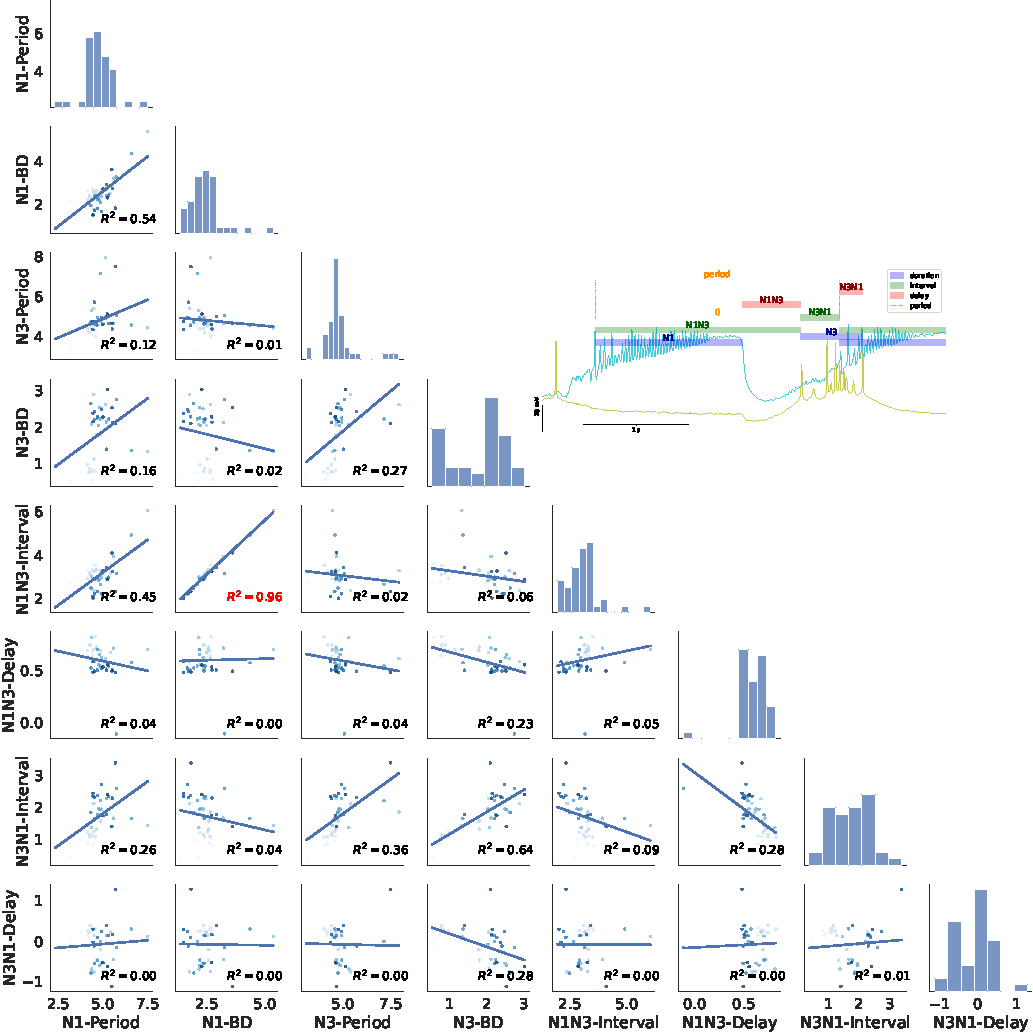
\includegraphics[width=0.48\textwidth]{./img/invariants/data/SUSSEX/CV1a_driven2/images/panel_with_pairplot.pdf}
	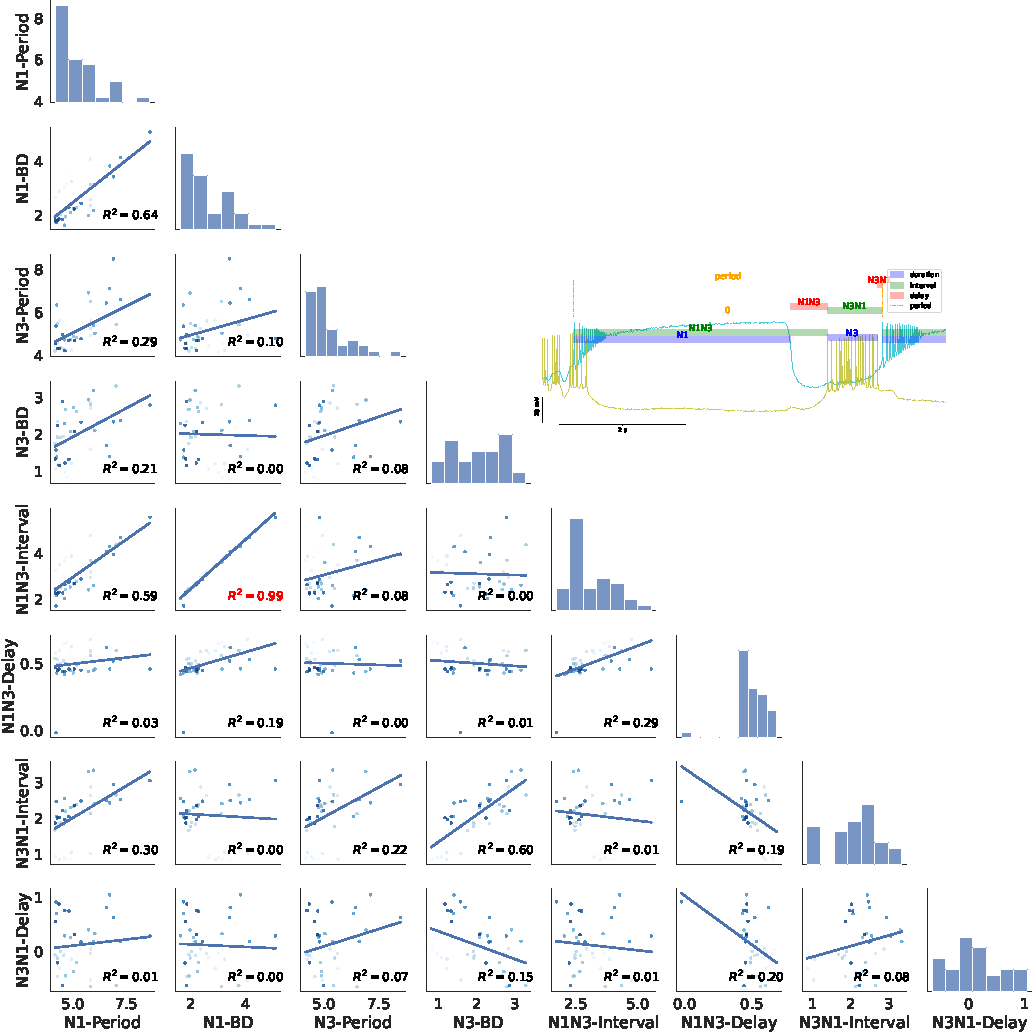
\includegraphics[width=0.48\textwidth]{./img/invariants/data/SUSSEX/CV1a_driven4/images/2phases/panel_with_pairplot.pdf}
	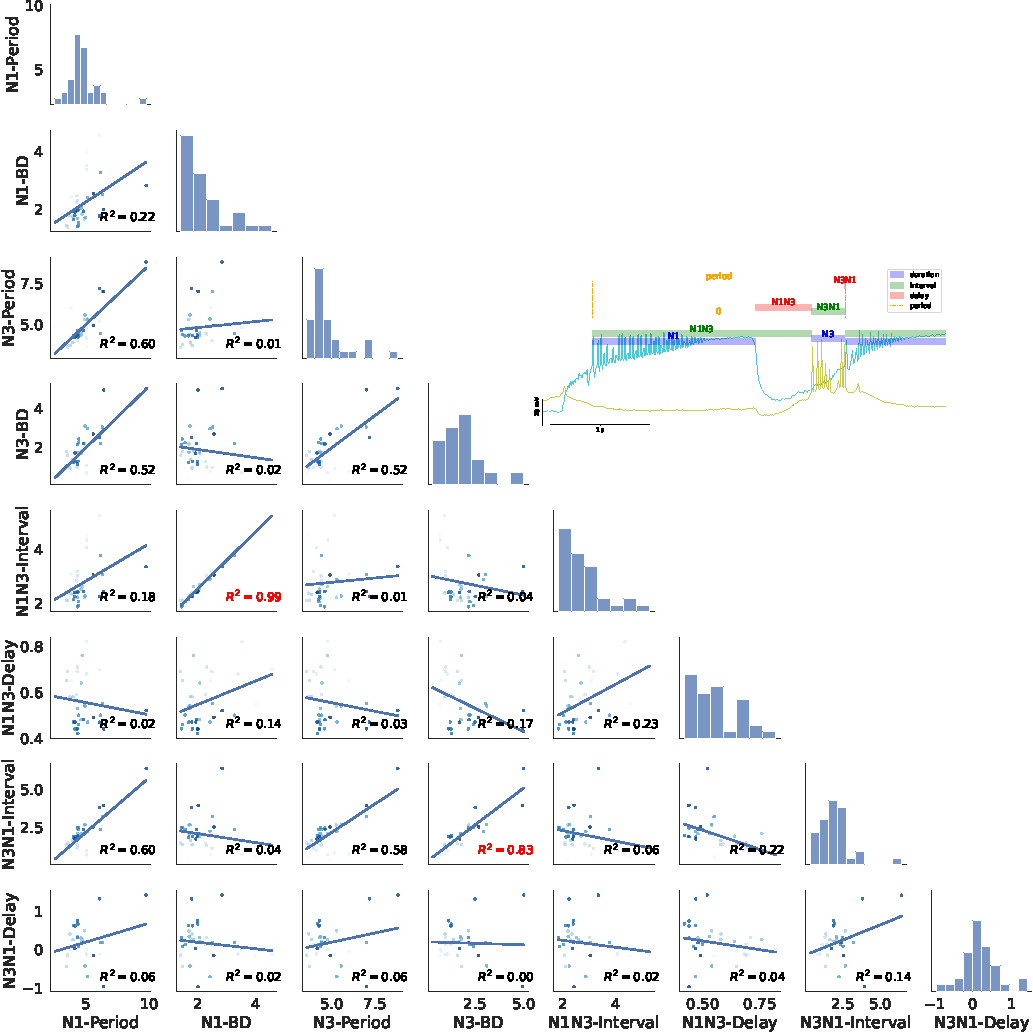
\includegraphics[width=0.48\textwidth]{./img/invariants/data/SUSSEX/CV1a_driven3/images/panel_with_pairplot.pdf}
	\caption{Panel of the pairplots for all possible combinations between the time intervals for two phases (N1 and N3) in the CPG recordings for the four examples of induced CV1a neuron modulation recordings.}
	\label{fig:cv1a pairplot comparison}
\end{figure}


\subsection{Invariants reseting}
There is another feature of the sequential dynamical invariants reported in \cite{elices_robust_2019}, that there is no relation of the time intervals cycle-by-cycle, which means there is no gradual modification of the rhythm but a sthocastic relation. We saw that in panels of this section, where most cases represented an time-interval duration with no linear relation when represented against the number of the cycle. In the model the study of this phenomena was not possible since the current ramp provided a gradual change of the time-intervals duration and so forcing all intervals correlated in a period to be also correlated in the next one (see Appendix Fig. \ref{fig:N1M stimulation pairplot reset}). 

In this subsection, we include several experimental examples of this relation in the examples presenting robust sequential dynamical invariants. We represent this "reset" with a pairplot gathering a cycle in the bottom triangle, and the relations of each interval with the next cycle represented in the upper triangle (Fig. \ref{fig:reset pairplot comparison}). There it can be appreciated that when comparing the intervals of one cycle to the next one, the correlations disappear, the most clear example for this is the first figure, for the spontaneous activiy, being all relations with a $R^2$ close to 0. In the two examples in the second row, the MLN stimulation and CV1a stimulation recordings, the are some strong correlations, but note that they are not in within the same intervals, e.g., the robust dynamical invariant in N1 burst duration with the period, disappear when comparing to the next cycle in both cases. The strong correlations are present between N1 and N3 periods and between N1 burst duration and N3 period. Both periods overlap, which can explain the relation. Therefore, cycle-by-cycle the variability is reseted, there is not a restriction in the variability where the duration of a interval pre-defines the next one, but a stochastic distribution of the activity that is compensated cycle-by-cycle. 

\begin{figure}[htbp]
	\centering
	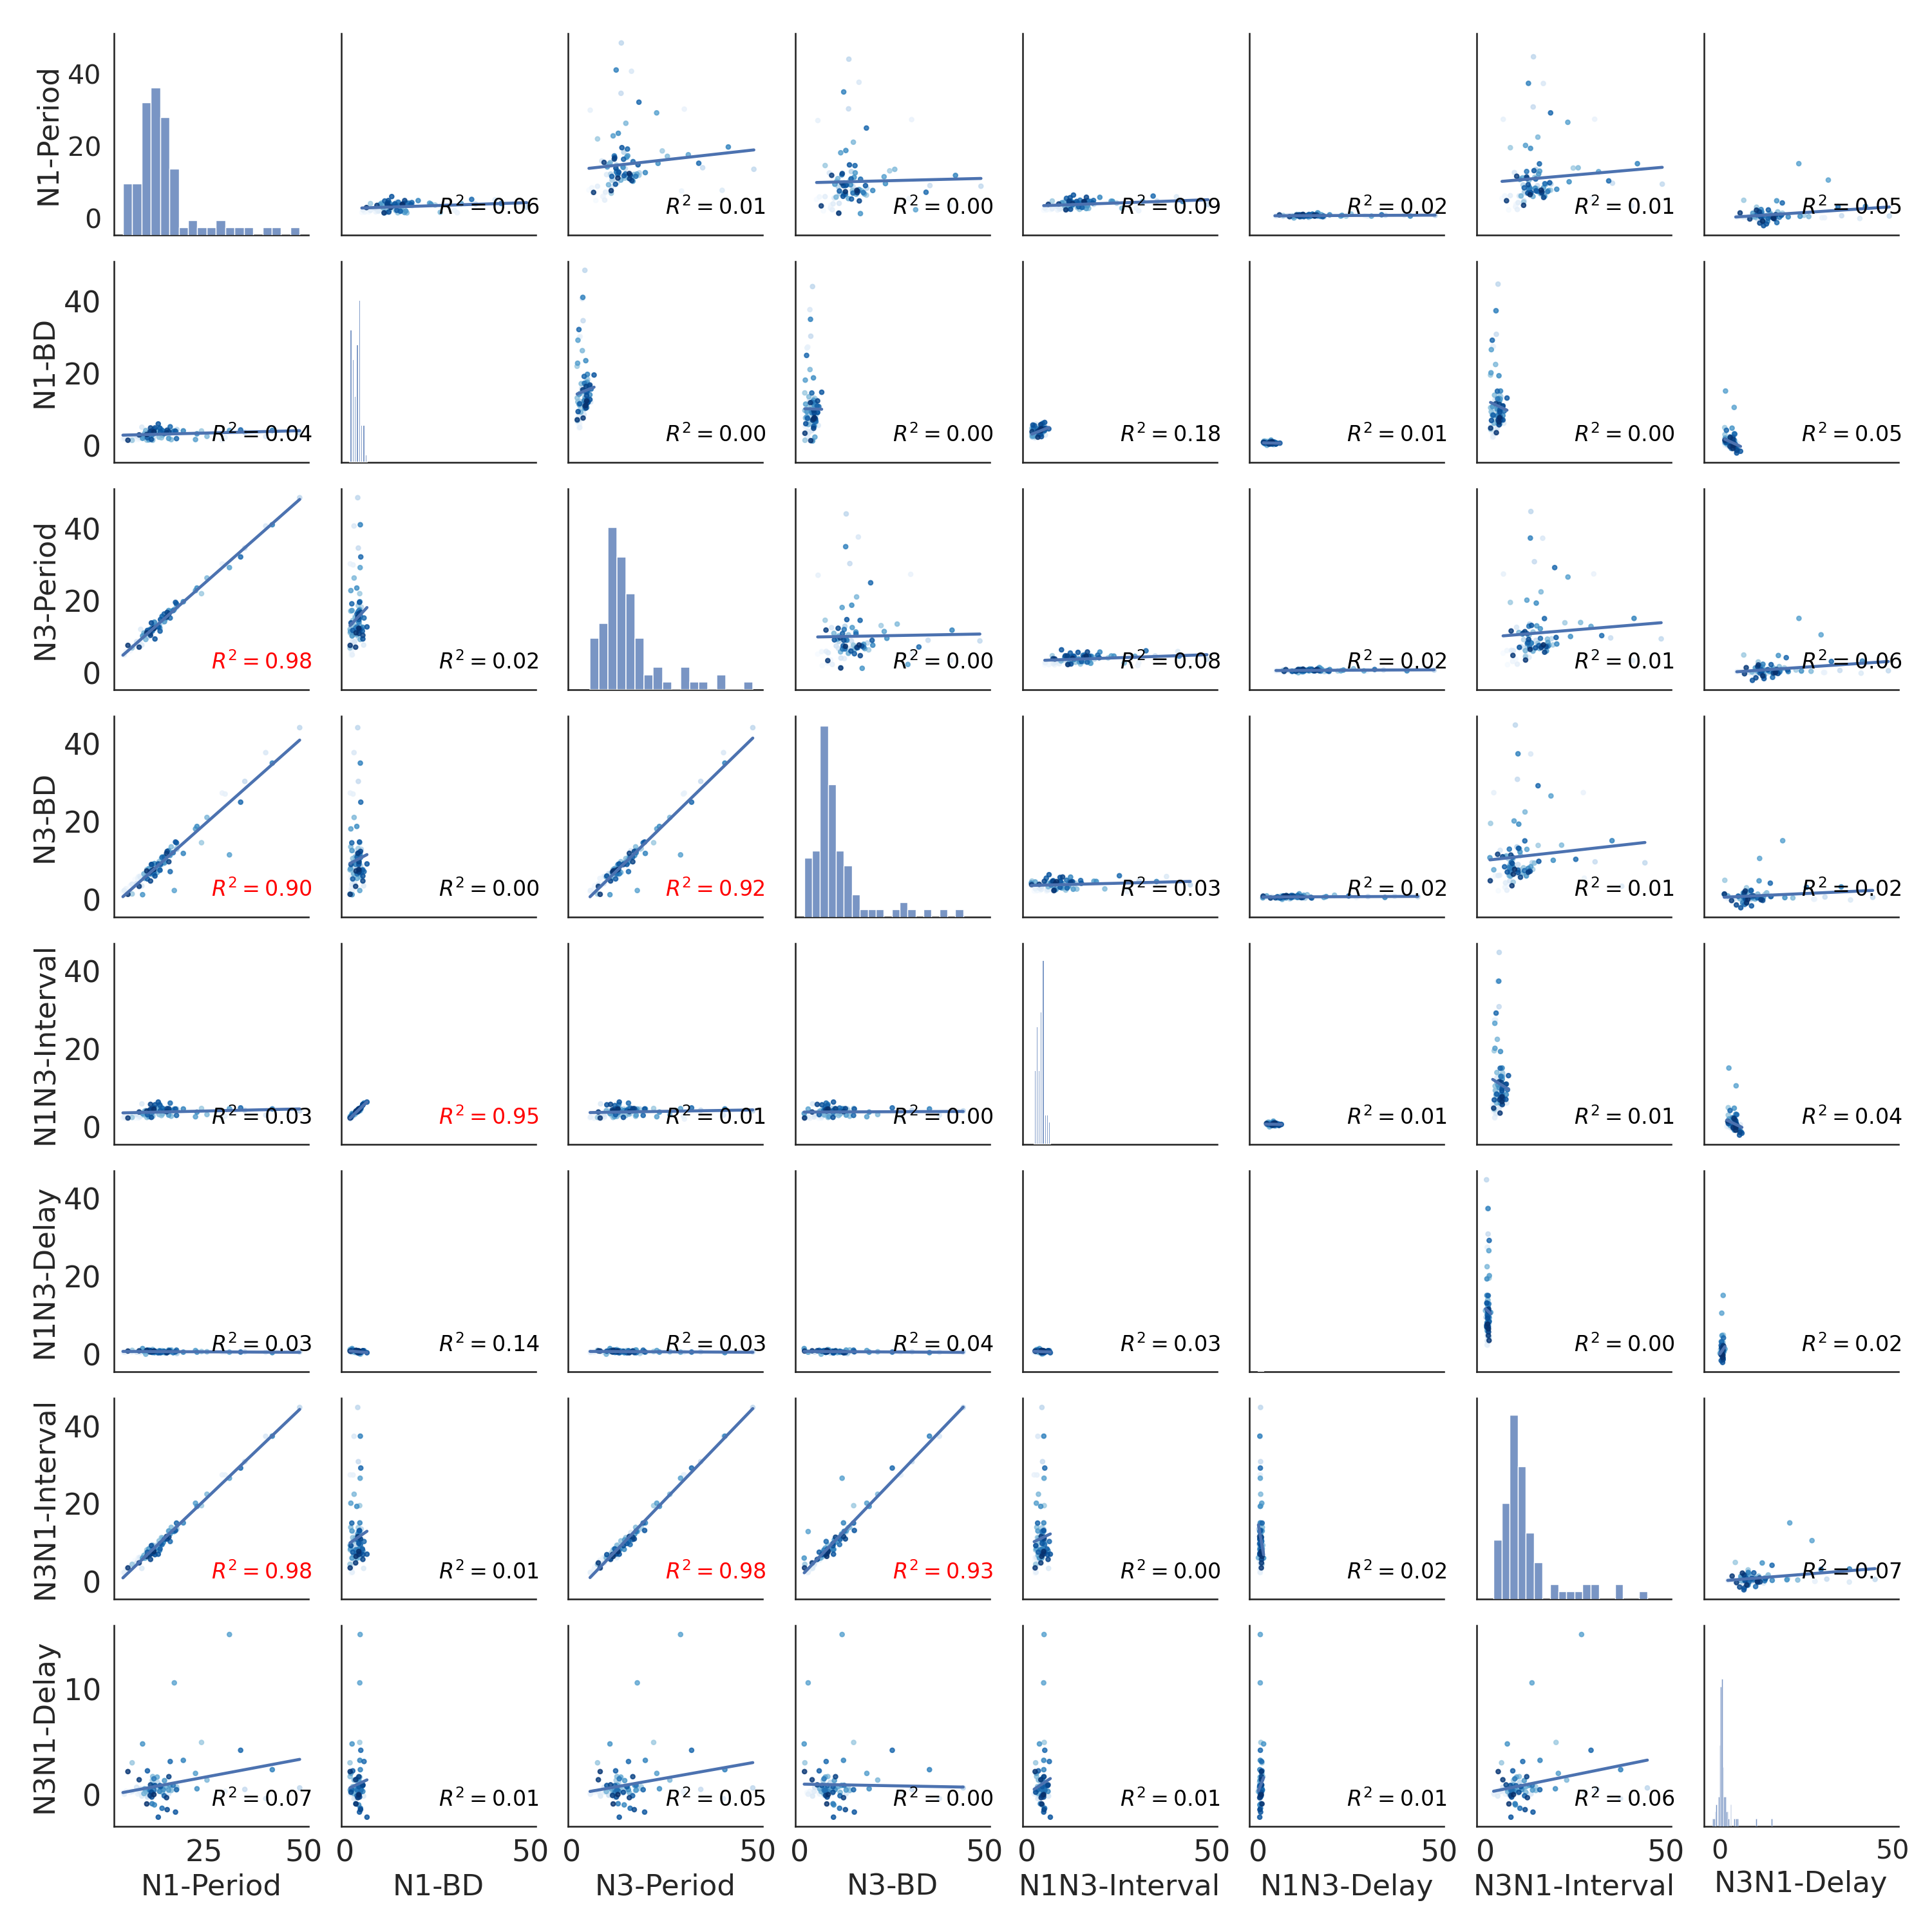
\includegraphics[width=0.49\textwidth]{./img/invariants/data/SUSSEX/prep2/images/2phases/_output_pairplot_reset.png}
	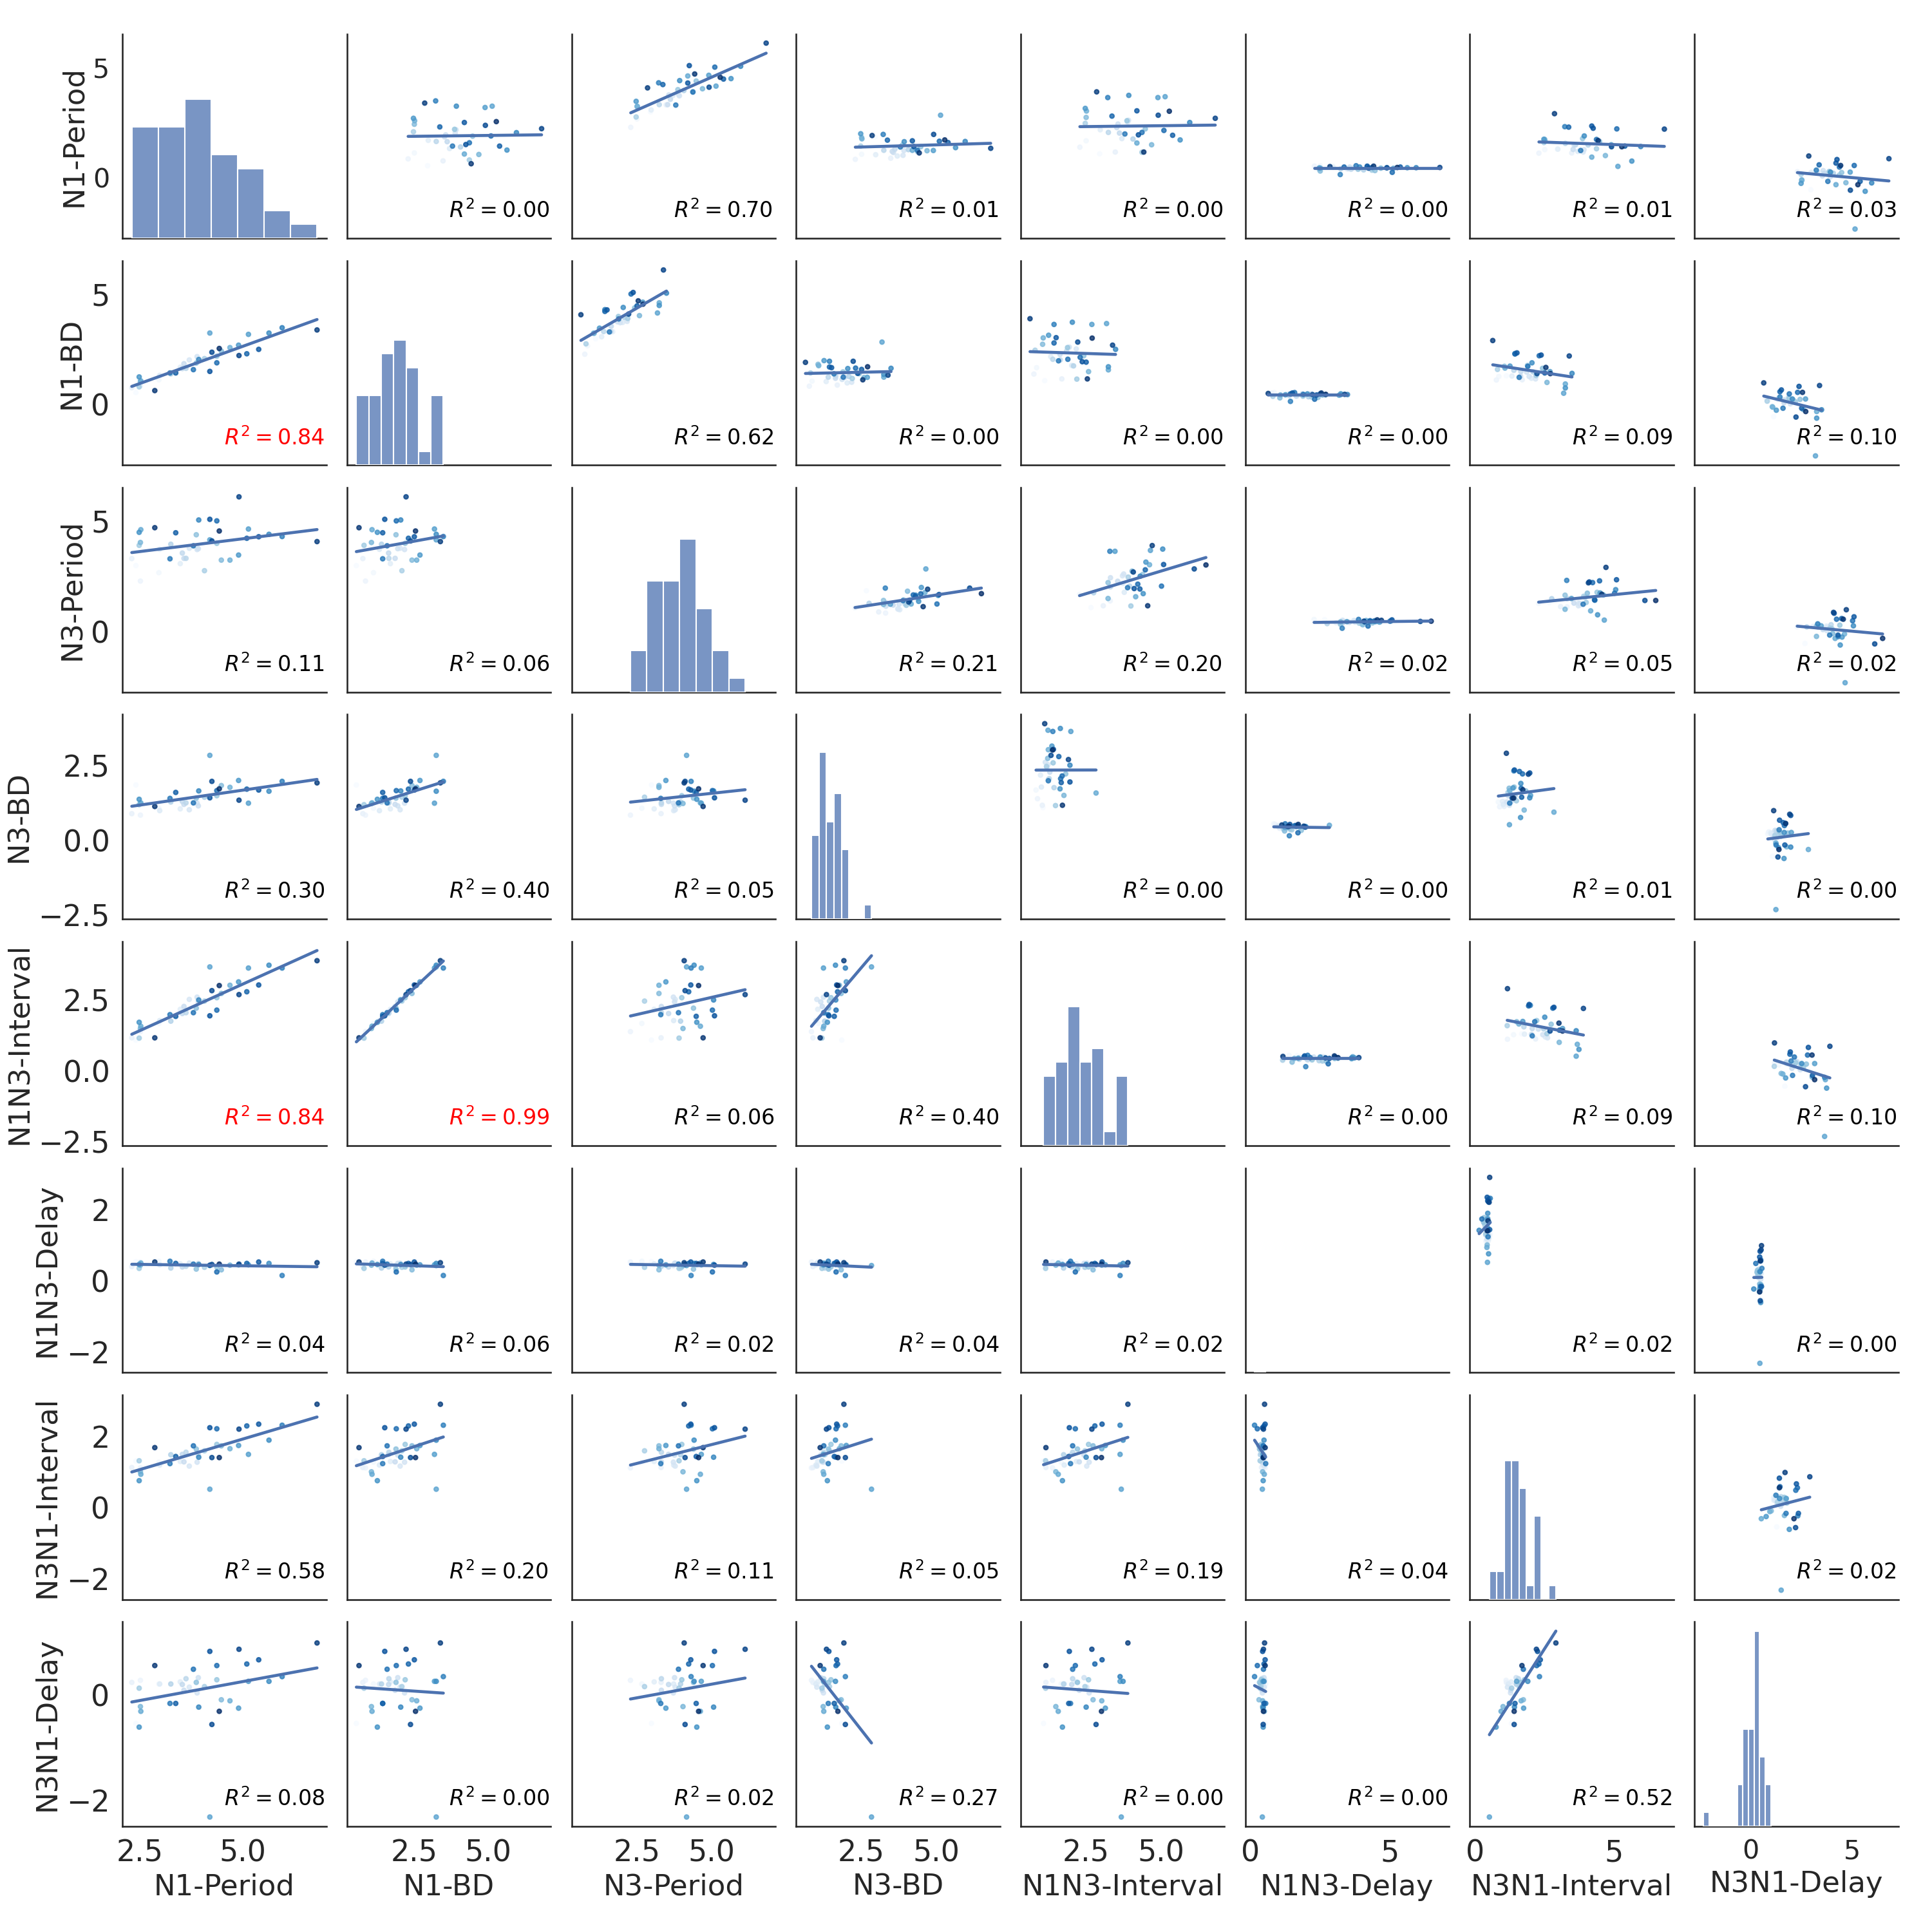
\includegraphics[width=0.49\textwidth]{./img/invariants/data/SUSSEX/SO_driven/images/_output_pairplot_reset.png}
	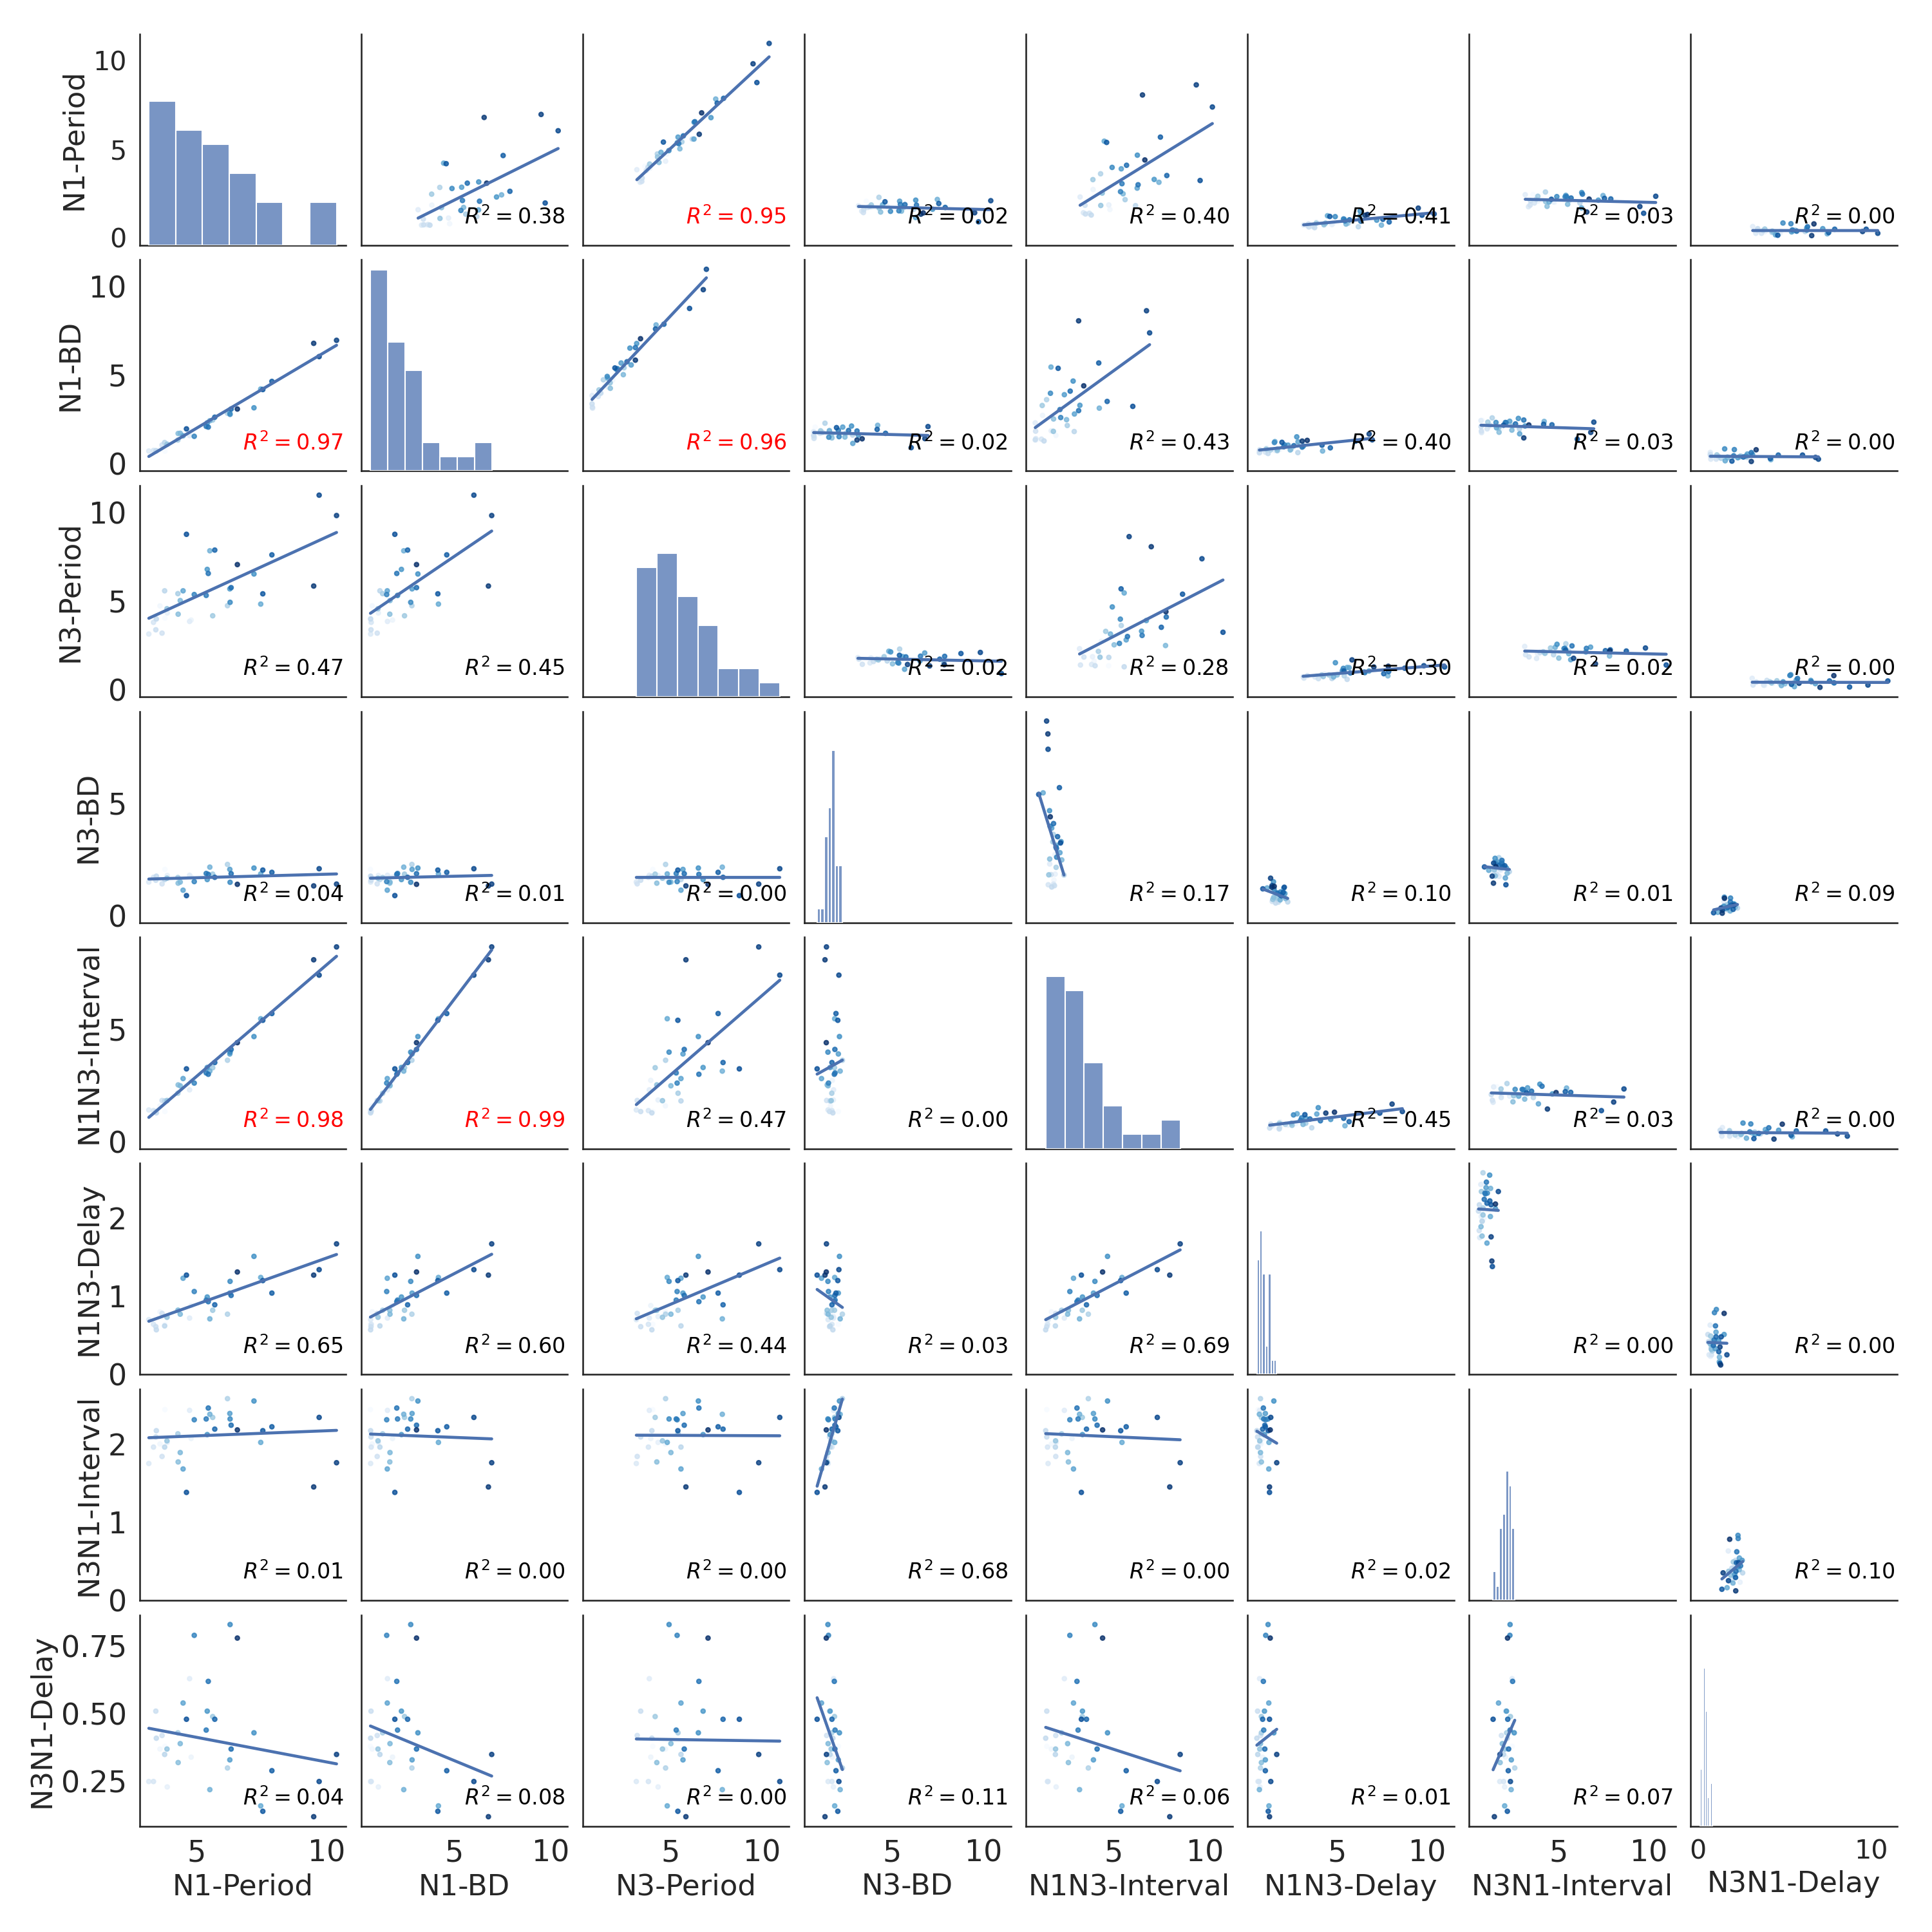
\includegraphics[width=0.49\textwidth]{./img/invariants/data/SUSSEX/MLN_driven/images/_output_pairplot_reset.png}
	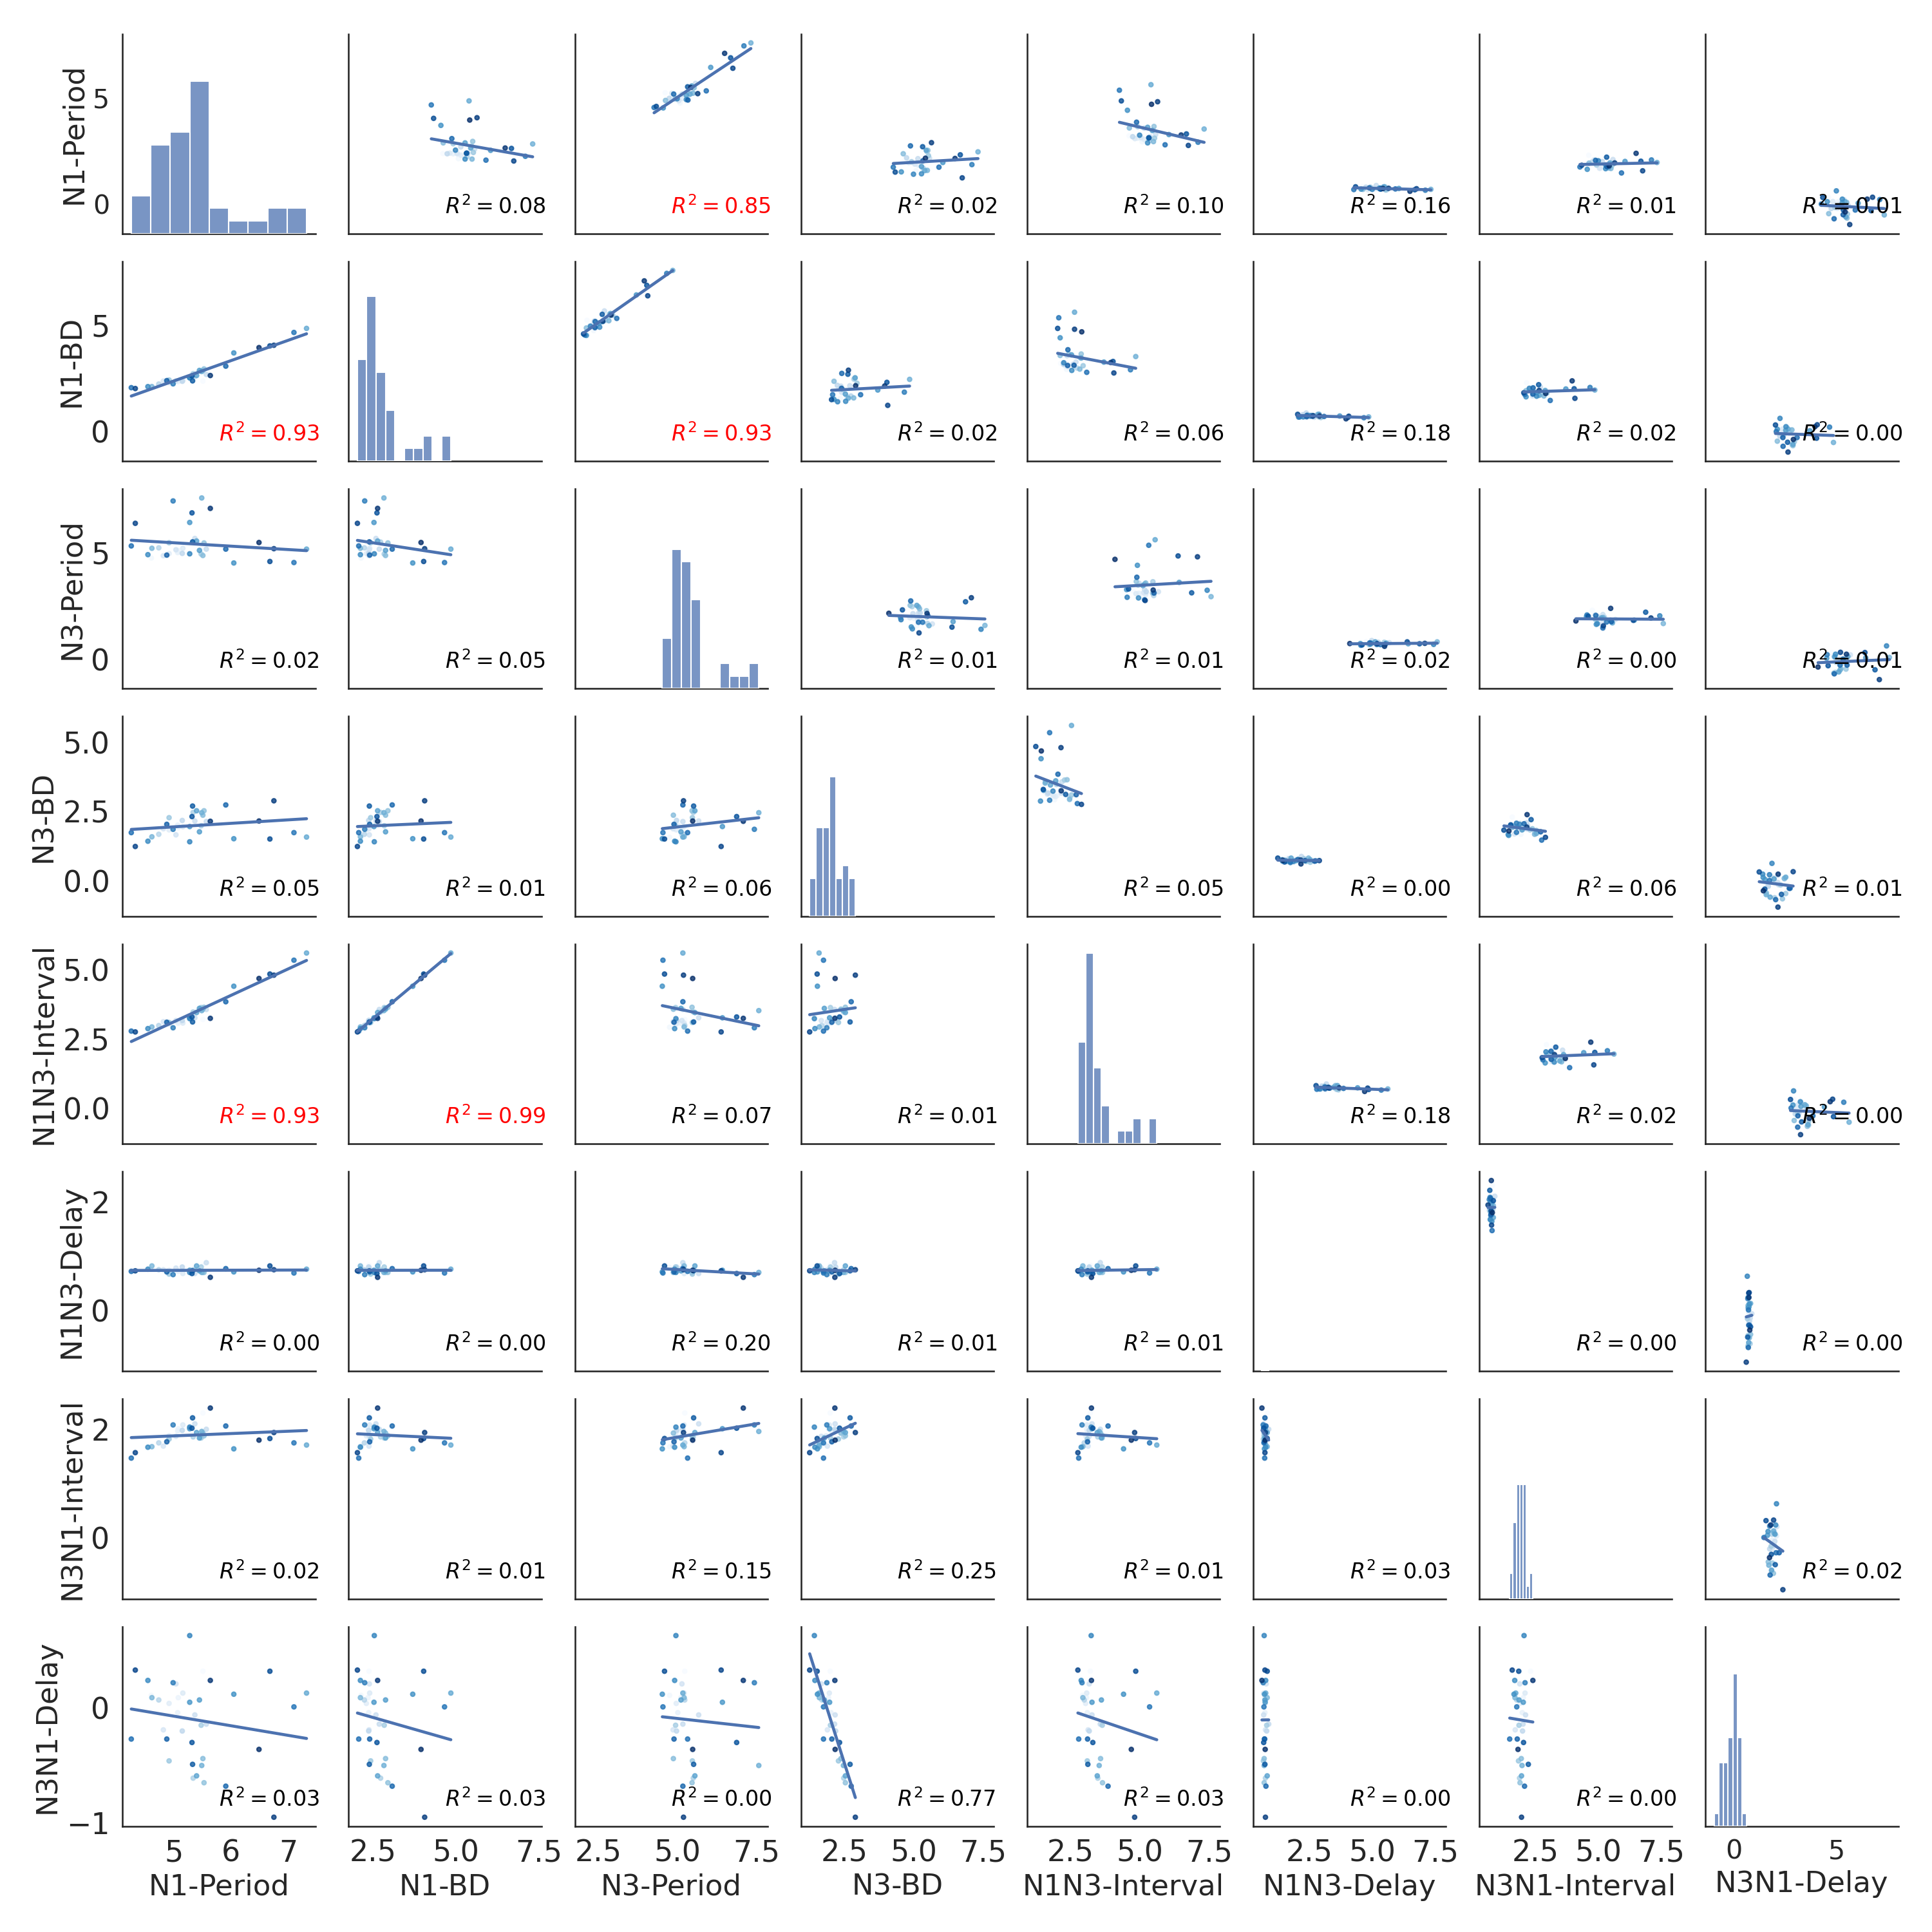
\includegraphics[width=0.49\textwidth]{./img/invariants/data/SUSSEX/CV1a_driven1/images/2phases/_output_pairplot_reset.png}
	\caption{Panel representing the reset cycle-by-cycle of dynamical invariants. For each pairplot the lower triangle represent a cycle and the upper triangle represents the intervals of that cycle against the intervals of next cycle. The examples showed here are from top left to right: Spontanoeus activity example 1 (Fig. \ref{fig:prep2 invariants}), SO induced modulation (Fig. \ref{fig:so induced invariants}), MLN stimulation (Fig. \ref{fig:mln stimulation}) and CVa1 stimulation (Fig. \ref{fig:cv1a 1 2phases})}
	\label{fig:reset pairplot comparison}
\end{figure}

\clearpage
\newpage
